% Created 2021-08-23 Mon 15:16
% Intended LaTeX compiler: xelatex
\documentclass[9pt]{report}
\usepackage{graphicx}
\usepackage{grffile}
\usepackage{longtable}
\usepackage{wrapfig}
\usepackage{rotating}
\usepackage[normalem]{ulem}
\usepackage{amsmath}
\usepackage{textcomp}
\usepackage{amssymb}
\usepackage{capt-of}
\usepackage[hidelinks]{hyperref}
\usepackage[a4paper, total={6in,9in}]{geometry}
         \usepackage{booktabs}
\usepackage{minted}
         \usepackage{tikz-cd}
\usepackage{circuitikz}
\usepackage{makecell}
\usepackage{tikz}
\usepackage{tabulary}
\usetikzlibrary{quotes,angles,positioning}
\usepackage{array}
\usepackage{parskip}
\usepackage[type={CC}, modifier={by-nc-sa}, version={4.0},]{doclicense}
\usepackage{forest}
\usepackage{sectsty}
\sectionfont{\fontsize{12}{15}\selectfont}
\subsectionfont{\fontsize{11}{11}\selectfont}
\setlength\parindent{0pt}
\usepackage{parskip}
\usepackage{pifont}
\makeatletter
\def\@makechapterhead#1{%
{\parindent \z@ \raggedright \normalfont
\ifnum \c@secnumdepth >\m@ne
\LARGE\bfseries \thechapter~
\fi
\interlinepenalty\@M
\LARGE \bfseries #1\par\nobreak
\vskip 10\p@
}}
\def\@makeschapterhead#1{%
{\parindent \z@ \raggedright
\normalfont
\interlinepenalty\@M
\Huge \bfseries  #1\par\nobreak
\vskip 10\p@
}}
\makeatother
\usepackage{colortbl}
\author{Nebhrajani A.V.}
\date{\today}
\title{MIT 6.001 1986 Video Notes}
\hypersetup{
 pdfauthor={Nebhrajani A.V.},
 pdftitle={MIT 6.001 1986 Video Notes},
 pdfkeywords={},
 pdfsubject={},
 pdfcreator={Emacs 27.2 (Org mode 9.4.4)},
 pdflang={English}}
\begin{document}

\maketitle
\tableofcontents

\newpage

\chapter{Prologue}
\label{sec:org403dd19}
\section{About}
\label{sec:orgfac3505}
These are my notes of the twenty SICP lectures of June 1986,
produced by Hewlett-Packard Television. These videos are available
under a Creative Commons license.

These notes aim to be concise and as example-heavy as possible. The
language used and referred to as ``Lisp'' is MIT-Scheme. These notes,
however, use the SICP language provided by Racket, a modern Scheme
dialect. This is because Racket's integration with Emacs and
Org mode is orders of magnitude better than MIT-Scheme's. In
general, all ``Lisp'' code looks exactly the same as in SICP, with the
exception of having to prefix some numbers with \texttt{\#i} to ensure
Racket treats them as imprecise.

\section{License}
\label{sec:orgd356acf}
\doclicenseThis

\chapter{Lecture 1A: Overview and Introduction to Lisp}
\label{sec:org32a93e4}

Computer science isn't really a science, and it isn't really about
computers. Computer science is the study of how-to or imperative
knowledge (as opposed to declarative knowledge). To illustrate the
difference, consider:

$$y = \sqrt{x} \mathrm{~such~that~} y^2=x, y \geq 0$$

This is declarative, in that we could recognize if \(y\) is the square
root of \(x\) given \(x\) and \(y\), but we're no closer to knowing how to
\emph{find} \(y\) if we are given \(x\). Imperative knowledge would look
like:

To find the square root \(y\) of \(x\):
\begin{itemize}
\item Make a guess \(g\).
\item If \(g^2\) is close enough to \(x\), \(y=g\).
\item Otherwise, make a new guess equal to the average of \(g\) and \(x/g\).
\end{itemize}

This method will eventually come up with a \(g\) close enough to the
actual square root \(y\) of \(x\).

Computer science focuses on this kind of imperative knowledge, and,
specifically, how to communicate that knowledge to a computer.

\section{Managing Complexity: Key Ideas of 6.001}
\label{sec:org9382d74}
Computer science is also about managing complexity, in that large
programs that you can't hold in your head should still be manageable
and easy to work with. We explore this theme in 6.001 by learning
three key ideas:

\begin{itemize}
\item Black-box abstractions
\item Conventional interfaces
\item Metalinguistic abstraction.
\end{itemize}


\section{Let's Learn Lisp}
\label{sec:orge65895a}
When learning a new language, always ask about its:
\begin{itemize}
\item Primitive elements,
\item Means of combination, and
\item Means of abstraction.
\end{itemize}

\subsection{Primitive Elements}
\label{sec:org0e97585}
These are numbers like 3, 17.4, or 5. Other primitives are
discussed later in the course.

\begin{minted}[]{racket}
4
17.4
5
\end{minted}

\begin{verbatim}
4
17.4
5
\end{verbatim}

\subsection{Means of Combination}
\label{sec:org91f1e09}
Lisp's numerical primitives can be combined with ``operations'' such
as addition, written in prefix notation.

\begin{minted}[]{racket}
(+ 3 17.4 5)
\end{minted}

\begin{verbatim}
25.4
\end{verbatim}


Other basic operations are provided by Lisp, such as
multiplication and division. Of course, combinations can be
combined recursively:

\begin{minted}[]{racket}
(+ 3 (* 5 6) 8 2)
\end{minted}

\begin{verbatim}
43
\end{verbatim}


This should show you the tree structure inherent in all of Lisp:
\begin{center}
\begin{forest}
[+
[* [5] [6]] [8] [2]]
\end{forest}
\end{center}

In Lisp, () is the application of an operation or function in
prefix notation.

\subsection{Means of Abstraction}
\label{sec:org6ed7f3a}

Abstraction can simply be done by naming things. Giving
complicated things a name prevents us from having to understand
how the thing the name refers to \emph{works}, and instead lets us
``abstractly'' use the name for our purposes.

\begin{minted}[]{racket}
(define a (* 5 5))
a
(* a a)
(define b (+ a (* 5 a)))
b
(+ a (/ b 5))
\end{minted}

\begin{verbatim}
25
625
150
55
\end{verbatim}


Now, it's often more useful to abstract away imperative how-to
knowledge. Consider:

\begin{minted}[]{racket}
(define (square x)
  (* x x))
\end{minted}

\begin{minted}[]{racket}

(square 10)
\end{minted}

\begin{verbatim}
100
\end{verbatim}


This defines \texttt{square} as a function taking a single argument \texttt{x},
and returning \texttt{(* x x)}. Note that this way of writing a define is
actually ``syntactic sugar'' for:

\begin{minted}[]{racket}
(define square
  (lambda (x)
    (* x x)))

(square 25)
\end{minted}

\begin{verbatim}
625
\end{verbatim}


\texttt{lambda (x)} means ``make a procedure that takes argument \texttt{x}''. The
second argument to lambda is the actual procedure body. The
\texttt{define} names this anonymous procedure \texttt{square}.

Just like we can use combinations recursively, so we can
abstractions. Consider:

\begin{minted}[]{racket}
(define (average x y)
  (/ (+ x y) 2))
\end{minted}

\begin{minted}[]{racket}


(define (mean-square x y)
  (average (square x)
           (square y)))

(mean-square 2 3)
\end{minted}

\begin{verbatim}
13/2
\end{verbatim}


Note the indentation: since Lisp is parenthesis heavy, we use
indentation. Good editors like Emacs should do this automatically.

\section{Case Analysis in Lisp}
\label{sec:org39881ba}

To represent functions like:
$$abs(x) = \begin{cases}
   -x & x<0\\
   0 & x = 0\\
   x & x > 0
   \end{cases}$$
Lisp needs some form of conditional execution. In Lisp, this
function would look like:

\begin{minted}[]{racket}
(define (abs x)
  (cond ((< x 0) (- x))
        ((= x 0) 0)
        ((> x 0) x)))
(abs -3)
(abs 0)
(abs 5)
\end{minted}

\begin{verbatim}
3
0
5
\end{verbatim}


\texttt{cond} takes any number of arguments. Each argument must be
structured as \texttt{(predicate) (consequent)}. If \texttt{predicate} is true,
we do the \texttt{consequent}. Otherwise, we don't. Lisp also provides a
way to write conditionals that only have two branches (an if-else):

\begin{minted}[]{racket}
(define (abs x)
  (if (< x 0)
      (- x)
      x))
\end{minted}

\begin{minted}[]{racket}

(abs -11)
(abs 0)
(abs 33)
\end{minted}

\begin{verbatim}
11
0
33
\end{verbatim}


\texttt{cond} and \texttt{if} are syntactical sugar for each other. The Lisp
implementation picks any one and defines the other in terms of it.

We now know most of Lisp. Lisp doesn't have \texttt{do...while} or \texttt{for},
since anything a loop can do can be done via recursion.

\section{Finding Square Roots}
\label{sec:orga714db0}

Remember our square root finding algorithm?

To find the square root \(y\) of \(x\):
\begin{itemize}
\item Make a guess \(g\).
\item If \(g^2\) is close enough to \(x\), \(y=g\).
\item Otherwise, make a new guess equal to the average of \(g\) and
\(x/g\).
\end{itemize}

Or, in Lisp,

\begin{minted}[]{racket}
(define (try g x)
  (if (good-enough? g x)
      g
      (try (improve g x) x)))
\end{minted}

This is a form of programming called ``wishful thinking'': we assume
\texttt{good-enough?} (good enough predicate) and \texttt{improve} are already
implemented. Now that we can try a guess and improve it till it's
good enough, we can write a simple square root function:

\begin{minted}[]{racket}
(define (sqrt x)
  (try 1 x))
\end{minted}

This function simply starts the guess at 1, then improves it. Let's
now write the functions we don't have:

\begin{minted}[]{racket}
(define (improve g x)
  (average g (/ x g)))
\end{minted}

\begin{minted}[]{racket}
(define (good-enough? g x)
  (< (abs (- (square g) x))
     0.00001))
\end{minted}

This tests if \(g^2\) is within 0.0001 of \(x\). Putting it all
together, we can finally try to find square roots:

\begin{minted}[]{racket}







(sqrt #i2)
(sqrt #i3)
(sqrt #i4)
\end{minted}

\begin{verbatim}
1.4142156862745097
1.7320508100147274
2.0000000929222947
\end{verbatim}


\begin{quote}
\textbf{Note:} The \texttt{\#i4} is Racket's syntax for using imprecise
(decimals) instead of precise (fractions). Ignore it, and treat it
as the number \texttt{4}.
\end{quote}

See that \texttt{try} actually runs a loop, but does so recursively,
calling itself every time the \texttt{if} condition fails to improve the
guess. Also note that these functions can all be nested inside the
square root function to hide them from the outer scope, thus:

\begin{minted}[]{racket}
(define (sqrt x)
  (define (good-enough? g)
    (define (square g)
      (* g g))
    (define (abs y)
      (if (< y 0)
          (- y)
          y))
    (< (abs (- (square g) x))
       0.0001))
  (define (improve g)
    (define (average y z)
      (/ (+ y z) 2))
    (average g (/ x g)))
  (define (try g)
    (if (good-enough? g)
        g
        (try (improve g))))
  (try 1))

(sqrt #i2)
\end{minted}

\begin{verbatim}
1.4142156862745097
\end{verbatim}


This program should also show you a tree-like dependency of the
functions, with each function containing the definitions of the
functions it depends on. For someone using \texttt{sqrt}, all the functions
within it are hidden.

\begin{center}
\begin{forest}
[\texttt{sqrt}
[\texttt{try}
[\texttt{good-enough?}
[\texttt{abs}] [\texttt{square}]]
[\texttt{improve}
[\texttt{average}]]
[\texttt{try}]]]
\end{forest}
\end{center}

This discipline of writing procedures is called lexical scoping.


\section{Inbuilt/Primitive Procedures Aren't Special}
\label{sec:org4f89703}

\begin{minted}[]{racket}

square
+
\end{minted}

\begin{verbatim}
#<procedure:square>
#<procedure:+>
\end{verbatim}

\chapter{Lecture 1B: Procedures and Processes, Substitution Model}
\label{sec:orgcbde629}

\section{Substitution Rule/Model}
\label{sec:orgf631423}
The substitution rule states that,

\begin{quote}
To evaluate an application:
\begin{itemize}
\item Evaluate the operator to get procedure.
\item Evaluate the operands to get arguments.
\item Apply procedure to arguments.
\begin{itemize}
\item Copy body of procedure.
\item Replace formal parameters with actual arguments.
\end{itemize}
\item Evaluate new body.
\end{itemize}
\end{quote}

Note that this isn't necessarily how the \emph{interpreter} evaluates a
Lisp application, but the substitution rule is a ``good enough''
model for our purposes.

\subsection{Kinds of Expressions in Lisp}
\label{sec:org9f13b27}
\begin{itemize}
\item Numbers (evaluate to ``themselves'')
\item Symbols (represent some procedure)
\item Combinations
\item \(\lambda\)-expressions (used to build procedures)
\item Definitions (used to name symbols)
\item Conditionals
\end{itemize}

We will focus our use of the substitution rule on the first three.
The last three are called ``special forms'', and we'll worry about
them later.

\subsection{Example}
\label{sec:org4e7dfb9}

Consider:

\begin{minted}[]{racket}

(define (sum-of-squares x y)
  (+ (square x) (square y)))

(sum-of-squares 3 4)
\end{minted}

\begin{verbatim}
25
\end{verbatim}


Let's try to apply the substitution rule to our application,

\begin{minted}[]{racket}
(sum-of-squares 3 4)
(+ (square 3) (square 4))
(+ (square 3) (* 4 4))
(+ (square 3) 16)
(+ (* 3 3) 16)
(+ 9 16)
25
\end{minted}

\section{Peano Arithmetic}
\label{sec:orge46d549}

\subsection{Simple Peano Addition}
\label{sec:orgf3413b8}
Peano arithmetic defines addition as:

\begin{minted}[]{racket}
(define (pa+ x y)
  (if (= x 0)
      y
      (pa+ (dec x) (inc y))))
\end{minted}

\begin{minted}[]{racket}

(pa+ 3 4)
\end{minted}

\begin{verbatim}
7
\end{verbatim}


Assume that \texttt{inc} and \texttt{dec} are primitives available that increment
and decrement the argument respectively. How is the procedure \texttt{pa+}
working? Let's apply the substitution rule.

\begin{minted}[]{racket}
(pa+ 3 4)
(if (= 3 0)
    4
    (pa+ (dec 3) (inc 4)))
(pa+ 2 5)
...
(pa+ 1 6)
...
(pa+ 0 7)
7
\end{minted}

We're skipping some steps, but the idea is that \texttt{x} keeps giving
one ``unit'' to \texttt{y} until it reaches zero. Then the sum is \texttt{y}.
Written with steps skipped:

\begin{minted}[]{racket}
(pa+ 3 4)
(pa+ 2 5)
(pa+ 1 6)
(pa+ 0 7)
7
\end{minted}

\subsection{Another Peano Adder}
\label{sec:orgf6f2cb1}
Consider:
\begin{minted}[]{racket}
(define (pb+ x y)
  (if (= x 0)
      y
      (inc (pb+ (dec x) y))))
\end{minted}


This is also a Peano adder: but it's implemented \emph{slightly}
differently syntax-wise, a few characters here and there. Let's
use the substitution rule to see how it works.

\begin{minted}[]{racket}
(pb+ 3 4)
(inc (pb+ 2 4))
(inc (inc (pb+ 1 4)))
(inc (inc (inc (pb+ 0 4))))
(inc (inc ((inc 4))))
(inc (inc 5))
(inc 6)
7
\end{minted}

See that it \emph{does} work:

\begin{minted}[]{racket}

(pb+ 3 4)
\end{minted}

\begin{verbatim}
7
\end{verbatim}


Now, consider how these two, \texttt{pa+} and \texttt{pb+}, are different. While
the \emph{procedures} do the same thing, the processes are wildly
different. Let's discuss their time and space complexity.
It should be obvious to you that the time complexity is the
vertical axis in the substitution rule application, since the
interpreter ``executes'' these instructions line by line. More lines
means more time.

In the case of \texttt{pa+}, the number of lines increases by 1 if you
increase input \texttt{x} by 1. Thus, the time complexity is \(O(x)\).
Similarly, in the case of \texttt{pb+}, the number of lines increases by
2 (once in the expansion, once in the contraction) when you
increase \texttt{x} by 1. Thus, it is also \(O(x)\).

Now, the horizontal axis shows us how much space is being used. In
the case of \texttt{pa+}, the space used is a constant. Thus, \(O(1)\). On
the other hand, see that \texttt{pb+} first \emph{expands} then \emph{contracts}.
The length of the maximum expansion increases by 1 if we increase
\(x\) by 1, since there's one more increment to do. Thus, \(O(x)\).

Now, we call a process like \texttt{pa+} \emph{linear iterative} and a process
like \texttt{pb+} \emph{linear recursive}.

\begin{center}
\begin{tabular}{lccl}
\toprule
Process & Time Complexity & Space Complexity & Type\\
\midrule
\texttt{pa+} & \(O(x)\) & \(O(1)\) & Linear iterative\\
\texttt{pb+} & \(O(x)\) & \(O(x)\) & Linear recursive\\
\bottomrule
\end{tabular}
\end{center}

Note that the \emph{process} \texttt{pa+} being iterative has nothing to do
with the implementation/definition of the \emph{procedure}, which is
recursive. Iteration refers to the constant space requirement.

\section{Differentiating Between Iterative and Recursive Processes}
\label{sec:orge0674e2}

One of the primary ways to differentiate between an iterative and
recursive process is to imagine what'd happen if you turned the
computer off, then resumed the current computation.

In a recursive process, we've lost some important information: how
deep into the recursion we are. In the \texttt{pb+} example, we wouldn't
know how many \texttt{inc}'s deep we are (information stored in the RAM by
the interpreter, not by the process), meaning that we can't return
the right value.

In an iterative process, we can pick up right where we left off,
since \emph{all} state information is contained by the process.

\section{Fibonacci Numbers}
\label{sec:orge7d0bae}

Fibonacci numbers are defined as:

$$F(x) =
   \begin{cases}
   0, & x = 0\\
   1, & x = 1\\
   F(x-1) + F(x-2), & \mathrm{otherwise}
   \end{cases}$$

The series itself is:
$$0,1,1,2,3,5,8,13,21,34,55\dots$$

Let's write a Lisp function to calculate the \(n\mathrm{th}\) Fibonacci
number, assuming 0 is the 0th.

\begin{minted}[]{racket}
(define (fib n)
  (if (< n 2)
      n
      (+ (fib (- n 1))
         (fib (- n 2)))))
(fib 10)
\end{minted}

\begin{verbatim}
55
\end{verbatim}


It works, that's true. But how \emph{well} does it work. Let's see. When
we call (say) \texttt{(fib 4)}, we also call \texttt{(fib 3)} and \texttt{(fib 2)}, both
of which also call \(\dots\) let's draw it:

\begin{center}
\begin{forest}
[\texttt{(fib 4)}
[\texttt{(fib 3)}
[\texttt{(fib 2)} [\texttt{(fib 1)} [1]] [\texttt{(fib 0)} [0]]]
[\texttt{(fib 1)} [1]]]
[\texttt{(fib 2)} [\texttt{(fib 1)} [1]] [\texttt{(fib 0)} [0]]]]
\end{forest}
\end{center}

A tree! Clearly, this is an exponential-time process, since
computing \(n+1\) takes exponentially more effort. Also note that
it's a pretty bad process, since we constantly recompute many
values. The space complexity is the maximum depth of the tree
(depth of recursion), which is at most \(n\). Therefore, the time
complexity is \(O(\mathrm{fib}(n))\) and space complexity is \(O(n)\).

It is useful to try and write an iterative Fibonacci with better
performance as an exercise.

\section{Towers of Hanoi}
\label{sec:org929d9f0}

From Wikipedia:

\begin{quote}
The Tower of Hanoi is a mathematical game or puzzle. It consists of
three rods and a number of disks of different diameters, which can
slide onto any rod. The puzzle starts with the disks stacked on one
rod in order of decreasing size, the smallest at the top, thus
approximating a conical shape. The objective of the puzzle is to
move the entire stack to the last rod, obeying the following simple
rules:

\begin{itemize}
\item Only one disk may be moved at a time.
\item Each move consists of taking the upper disk from one of the
stacks and placing it on top of another stack or an empty rod.
\item No disk may be placed on top of a disk that is smaller than it.
\end{itemize}
\end{quote}

Let's try to solve Hanoi for 4 disks, from rod A to rod C. Again
--- ``wishful thinking''. Let's assume that we know how to solve for
3 disks. To solve, we'd take the top 3 disks, put it on the spare
rod B. Then, we'd take the fourth and largest disk, and put it on
destination rod C. Finally, we'd move the three disk pile from B
to C. Solved!

But wait --- to solve the 3 disk case, let's assume we know how to
solve the 2 disk case.

To solve the 2 disk case, we should know how
to solve the one disk case, which is just moving a disk from a rod
to another.

Or, in Lisp,

\begin{minted}[]{racket}
(define (move n from to spare)
  (cond ((= n 1) (display "Move disk at rod ")
                 (display from)
                 (display " to rod ")
                 (display to)
                 (display ".\n"))
        (else
         (move (- n 1) from spare to)
         (move 1 from to spare)
         (move (- n 1) spare to from))))

(move 4 "A" "C" "B")
\end{minted}

\begin{verbatim}
Move disk at rod A to rod B.
Move disk at rod A to rod C.
Move disk at rod B to rod C.
Move disk at rod A to rod B.
Move disk at rod C to rod A.
Move disk at rod C to rod B.
Move disk at rod A to rod B.
Move disk at rod A to rod C.
Move disk at rod B to rod C.
Move disk at rod B to rod A.
Move disk at rod C to rod A.
Move disk at rod B to rod C.
Move disk at rod A to rod B.
Move disk at rod A to rod C.
Move disk at rod B to rod C.
\end{verbatim}

Note, of course, that this procedure too, is an exponential time
procedure. However, any procedure for Hanoi will be exponential
time, since for \(n\) disks, Hanoi requires \(2^{n-1}\) moves. Even if
you compute every move in \(O(1)\) (which we do, since it's just a
print), the complexity will be \(O(2^n)\).

\section{Iterative Fibonacci}
\label{sec:org96b0429}

\begin{minted}[]{racket}
(define (iter-fib n a b)
  (if (= n 1)
      b
      (iter-fib (dec n) b (+ a b))))

(define (fib n)
  (iter-fib n 0 1))

(fib 10)
\end{minted}

\begin{verbatim}
55
\end{verbatim}

\chapter{Lecture 2A: Higher-Order Procedures}
\label{sec:orge150a3f}

\section{Abstracting Procedural Ideas}
\label{sec:org00551d1}

Consider the functions and their respective (recursive) procedures:

$$\sum_{i=a}^{b} i$$

\begin{minted}[]{racket}
(define (sum-int a b)
  (if (> a b)
      0
      (+ a
         (sum-int (inc a) b))))

(sum-int 0 10)
\end{minted}

\begin{verbatim}
55
\end{verbatim}


$$\sum_{i=a}^{b} i^{2}$$

\begin{minted}[]{racket}

(define (sum-sq a b)
  (if (> a b)
      0
      (+ (square a)
         (sum-sq (inc a) b))))

(sum-sq 0 4)
\end{minted}

\begin{verbatim}
30
\end{verbatim}


$$\sum_{i=a_{\mathrm{~by~}4}}^{b} \frac{1}{i(i+2)}$$

Note that this series estimates \(\pi /8\).

\begin{minted}[]{racket}
(define (sum-pi a b)
  (if (> a b)
      0
      (+ (/ 1
            (* a (+ a 2)))
         (sum-pi (+ a 4) b))))

(* 8 (sum-pi #i1 #i1000000))
\end{minted}

\begin{verbatim}
3.141590653589793
\end{verbatim}



See that the commonality between these procedures comes from the
fact that the notion of ``summation'' from \texttt{a} to \texttt{b} is the same,
but the \emph{function} being summed is different in each case. Or, in
general form:

\begin{minted}[]{racket}
(define (<name> a b)
  (if (> a b)
      0
      (+ (<term> a)
         (<name> (<next> a) b))))
\end{minted}

The way to solve this is by writing a procedure \texttt{sum}, which has
available to it two procedures \texttt{term} and \texttt{next}. We supply these
as arguments. Consider:

\begin{minted}[]{racket}
(define (sum term a next b)
  (if (> a b)
      0
      (+ (term a)
         (sum term (next a) next b))))
\end{minted}

When we call \texttt{sum} recursively, see that we pass to it the \emph{same
procedures} \texttt{term} and \texttt{next}, along with \texttt{b} and the next value of
\texttt{a}. Now, it is easy to define \texttt{sum-int}, \texttt{sum-sq}, and \texttt{sum-pi}
using \texttt{sum}, thus:

\begin{minted}[]{racket}

(define (sum-int a b)
  (define (identity x) x)
  (sum identity
       a
       inc
       b))

(sum-int 0 10)
\end{minted}

\begin{verbatim}
55
\end{verbatim}


\texttt{identity} is the function \(p(x) = x\).

\begin{minted}[]{racket}


(define (sum-sq a b)
  (sum square
       a
       inc
       b))

(sum-sq 0 4)
\end{minted}

\begin{verbatim}
30
\end{verbatim}


\begin{minted}[]{racket}

(define (sum-pi a b)
  (sum (lambda (x)
         (/ 1
            (* x (+ x 2))))
       a
       (lambda (x) (+ x 4))
       b))

(* 8 (sum-pi #i1 #i1000000))
\end{minted}

\begin{verbatim}
3.141590653589793
\end{verbatim}


Recall that \texttt{lambda} means ``make a procedure'' that is nameless. In
\texttt{sum-pi}, we choose to give \texttt{sum} anonymous functions as arguments
instead of defining our own, because there's no reason to name a
procedure we won't later use.

The big advantage of abstracting away \texttt{sum} this way is that in
case we want to implement it in a different way, we merely have to
change the implementation of one function (\texttt{sum}) and not that of
the three functions that use it. In fact, those functions can
remain exactly the same.

Here's another implementation of \texttt{sum}. See that \texttt{sum-pi} still
works without changes, because it doesn't care about how \texttt{sum} is
implemented as long as the argument number and order remains
constant.

\begin{minted}[]{racket}
(define (sum term a next b)
  (define (iter j ans)
    (if (> j b)
        ans
        (iter (next j)
              (+ (term j)
                 ans))))
  (iter a 0))

(define (sum-pi a b)
  (sum (lambda (x)
         (/ 1
            (* x (+ x 2))))
       a
       (lambda (x) (+ x 4))
       b))

(* 8 (sum-pi #i1 #i1000000))
\end{minted}

\begin{verbatim}
3.1415906535898936
\end{verbatim}

\section{More on Square Roots}
\label{sec:org91033ed}

Recall our square root procedure. When seen in Lisp code, it's not
very clear what it's doing, or how it's working.

\begin{minted}[]{racket}
(define (sqrt x)
  (define (good-enough? g)
    (define (square g)
      (* g g))
    (define (abs y)
      (if (< y 0)
          (- y)
          y))
    (< (abs (- (square g) x))
       0.0001))
  (define (improve g)
    (define (average y z)
      (/ (+ y z) 2))
    (average g (/ x g)))
  (define (try g)
    (if (good-enough? g)
        g
        (try (improve g))))
  (try 1))
\end{minted}

\begin{minted}[]{racket}

(sqrt #i2)
\end{minted}

\begin{verbatim}
1.4142156862745097
\end{verbatim}


Let's use higher-order procedure abstraction to make it clearer.

\subsection{Fixed Points}
\label{sec:org7dc6a2d}

Recall that the algorithm itself relies on writing a function

$$f\colon y\mapsto \frac{y+\frac{x}{y}}{2}$$

Note that this works because \(f(\sqrt{x}) = \sqrt{x}\):

$$f(\sqrt{x})=\frac{\sqrt{x}+\frac{x}{\sqrt{x}}}{2} = \frac{2\sqrt{x}}{2} = \sqrt{x}$$

See that this is \emph{actually} an algorithm for finding a fixed point
of a function \(f\), which is defined as finding the point where
\(f(z)=z\). This algorithm is merely an instance of a function \(f\)
whose fixed point happens to be the square root.

\begin{quote}
For some functions, the fixed point can be found by iterating it.
\end{quote}

This is the top-level abstraction we'll write a function for.
First, let's see how we'd write a square-root function by wishful
thinking:

\begin{minted}[]{racket}

(define (sqrt x)
  (fixed-point
   (lambda (y) (average (/ x y)
                        y))
   1))
\end{minted}

Now writing \texttt{fixed-point}:

\begin{minted}[]{racket}

(define (fixed-point f start)
  (define (close-enough-p x y)
    (< (abs (- x y))
       0.00001))
  (define (iter old new)
    (if (close-enough-p old new)
        new
        (iter new (f new))))
  (iter start (f start)))
\end{minted}

Let's try it out!

\begin{minted}[]{racket}


(sqrt #i2)
\end{minted}

\begin{verbatim}
1.4142135623746899
\end{verbatim}

\subsection{Damping Oscillations}
\label{sec:org7e8f3d3}

A fair question when seeing the function
$$f_1\colon y\mapsto \frac{y+\frac{x}{y}}{2}$$
is why another function
$$f\colon y\mapsto \frac{x}{y}$$
wouldn't work in its place. This question is best
answered by trying to find its fixed point by iteration. Let's try
to find it for \(x=2\), starting at \(y=1\). Then,

$$f(1) = \frac{2}{1} = 2$$
$$f(2) = \frac{2}{2} = 1$$
$$f(1) = \frac{2}{1} = 2$$
$$f(2) = \frac{2}{2} = 1$$
$$~\dots$$

It seems that instead of converging, this function is
\emph{oscillating} between two values. We know that it's easy to fix
this: we have to damp these oscillations. The most natural way to
do this is to take the average of successive values \(y\) and
\(f(y)\). A \texttt{sqrt} function that uses average damping would be:

\begin{minted}[]{racket}

(define (sqrt x)
  (fixed-point
   (avg-damp (lambda (y) (/ x y)))
   1))
\end{minted}

The \texttt{avg-damp} function takes in a procedure, creates an average damping
procedure, and returns it. Or, in Lisp:

\begin{minted}[]{racket}

(define avg-damp
  (lambda (f)
    (lambda (x) (average (f x) x))))
\end{minted}

It is worth discussing how \texttt{avg-damp} works. It is defined as a
procedure which takes the argument of a function \texttt{f}. It then
returns an anonymous procedure which takes an argument \texttt{x}, and
computes the average of \(f(x)\) and \(x\). This is finally the
highest level of abstraction we can reach for the \texttt{sqrt}
algorithm --- finding the fixed point of a damped oscillating
function.

Using the \texttt{sqrt} function,

\begin{minted}[]{racket}


(sqrt #i2)
\end{minted}

\begin{verbatim}
1.4142135623746899
\end{verbatim}

\section{Newton's Method}
\label{sec:org7f3a90d}

Newton's method is used to find the zeros of a function (\(y \ni
   f(y)=0\)). To use it, start with some guess \(y_0\). Then,

$$y_{n+1} = y_n - \frac{f(y_n)}{f'(y_n)}$$

where $$f'(y) = \frac{\mathrm{d}f(y)}{\mathrm{d}y}$$

We can, of course, find the zero of the square root finding function
\(f(y) =  x-y^2\) using Newton's method. Note that Newton's method
\emph{itself} is based on fixed points, since it aims to find a fixed
point where \(y_{n+1}\approx y_n\).

Defining \texttt{sqrt}:

\begin{minted}[]{racket}

(define (sqrt x)
  (newton (lambda (y) (- x (square y)))
          1))
\end{minted}

We pass to \texttt{newton} a function \(f(y)=x-y^2\), since its zero is \(x=y^2\).

\begin{minted}[]{racket}

(define (newton f guess)
  (define df (deriv f))
  (fixed-point
   (lambda (x) (- x
                  (/ (f x)
                     (df x))))
   guess))
\end{minted}


It is important to note that defining \texttt{df} to be \texttt{(deriv f)} once
prevents wasteful recomputation of \texttt{df} every time \texttt{fixed-point}
calls itself.

Of course, we now have to define a derivative function. We can
simply use the standard limit definition to find it numerically:

$$f'(x) = \lim_{\Delta x\to 0} \frac{f(x+\Delta x) - f(x)}{\Delta
   x}$$

Or, in Lisp,

\begin{minted}[]{racket}
(define dx 0.0000001)

(define deriv
  (lambda (f)
    (lambda (x)
      (/ (- (f (+ x dx))
            (f x))
         dx))))


\end{minted}

This function returns a function which is the derivative of \texttt{f},
and can be used as such. Consider:

\begin{minted}[]{racket}

((deriv (lambda (x) (* x x x))) 2)
\end{minted}

\begin{verbatim}
12.000000584322379
\end{verbatim}


Which is the expected value of differentiating \(x^{3}\) w.r.t \(x\)
(\(3x^2\)) and evaluating at 2.

Testing out our \texttt{sqrt} function:

\begin{minted}[]{racket}



(sqrt #i2)
\end{minted}

\begin{verbatim}
1.4142135623747674
\end{verbatim}

\section{Procedures are First-Class Citizens}
\label{sec:org8a23c8e}

This means that procedures can be:
\begin{itemize}
\item Named using variables.
\item Passed as arguments to procedures.
\item Returned as values from procedures.
\item Included in data structures.
\end{itemize}

\chapter{Lecture 2B: Compound Data}
\label{sec:orgb8d3cb2}

Consider our \texttt{sqrt} function that uses \texttt{good-enough?}. What we did
while writing \texttt{sqrt} is assume the existence of \texttt{good-enough?}.
That is, we divorced the task of building \texttt{sqrt} from the task of
implementing its parts.

Let's do this for data.

\section{Rational Number Arithmetic}
\label{sec:orgad300f5}

Let's design a system which can add fractions:
$$\frac{1}{2}+\frac{1}{4}=\frac{3}{4}$$
and multiply them:
$$\frac{3}{4}\times \frac{2}{3} = \frac{1}{2}$$

The \emph{procedures} for these two tasks are well known to most people:

$$\frac{n_1}{d_1} + \frac{n_2}{d_2} = \frac{n_1d_2+n_2d_2}{d_1d_2}$$
and
$$\frac{n_1}{d_1} \times \frac{n_2}{d_2} = \frac{n_1n_2}{d_1d_2}$$

\subsection{Abstraction}
\label{sec:orgc32dfa8}
We don't know, however, how to represent this data in a Lisp
procedure. Let's use our powerful ``wishful thinking'' strategy.
Assume that we have the following procedures available to us:

\begin{itemize}
\item A constructor \texttt{(make-rat n d)} which makes a fraction with
numerator \texttt{n} and denominator \texttt{d}.
\item Two selectors:
\begin{itemize}
\item \texttt{(numer x)} which takes in a fraction \texttt{x} and returns its
numerator.
\item \texttt{(denom x)} which takes in a fraction \texttt{x} and returns its
denominator.
\end{itemize}
\end{itemize}

Then, our procedures are easy to write:

\begin{minted}[]{racket}
(define (+rat x y)
  (make-rat
   (+ (* (numer x) (denom y))
      (* (numer y) (denom x)))
   (* (denom x) (denom y))))

(define (*rat x y)
  (make-rat
   (* (numer x) (numer y))
   (* (denom x) (denom y))))
\end{minted}

Why do we need this data object abstraction anyway? We could very
well define \texttt{+rat} to take in four numbers, two numerators and two
denominators. But to return, we can't return \emph{both} numerator and
denominator. We now have to define two summation functions, one for
the numerator and one for the denominator, and somehow keep track
of the fact that one of these numbers is the numerator and the other
the denominator. Furthermore, when applying more complex operations
like:

\begin{minted}[]{racket}
(*rat (+rat x y)
      (+rat s t))
\end{minted}

The data abstraction helps. If it weren't there, we'd have to
maintain some temporary registers to store the numerator and
denominator values of the \texttt{+rat} operations into, then pass them to
\texttt{*rat}.

Worse than confusing the program, such a design philosophy would
confuse us, the programmers.

\subsection{Data Object Creation}
\label{sec:org596db44}

The glue we use to stick two numbers together is provided by three
Lisp primitives:
\begin{itemize}
\item A constructor \texttt{cons}, which generates an ordered pair.
\item Two selectors:
\begin{itemize}
\item \texttt{car}, which selects the first element of the pair, and
\item \texttt{cdr}, which selects the second element of the pair.
\end{itemize}
\end{itemize}

In use,
\begin{minted}[]{racket}
(define x (cons 1 2))
(car x)
(cdr x)
\end{minted}

\begin{verbatim}
1
2
\end{verbatim}


We can now write the procedures that we'd deferred writing
earlier:

\begin{minted}[]{racket}
(define (make-rat x y)
  (cons x y))

(define (numer x)
  (car x))

(define (denom x)
  (cdr x))
\end{minted}

\begin{minted}[]{racket}



(define x (make-rat 1 2))
(define y (make-rat 1 4))
(define z (+rat x y))
(numer z)
(denom z)
\end{minted}

\begin{verbatim}
6
8
\end{verbatim}


Agh. We forgot to reduce results to the simplest form. We can
easily include this in the \texttt{make-rat} procedure:\footnote{\texttt{let} is a Lisp primitive which takes as its first argument a
series of definitions, and second input a series of applications that may
use these definitions. The trick is that these definitions are only
valid in the body (second argument) of \texttt{let}, effectively creating a
local namespace.}

\begin{minted}[]{racket}
(define (make-rat x y)
  (let ((g (gcd x y)))
    (cons (/ x g)
          (/ y g))))

(define (numer x)
  (car x))

(define (denom x)
  (cdr x))
\end{minted}

Note that we could shift the \texttt{gcd} bit to functions \texttt{numer} and
\texttt{denom}, which would display the simplest form at access time
rather than creation time. Deciding between the two is a matter of
system efficiency: a system which displays often should use
creation time simplification, while a system which creates many
fractions should use access time simplification.
We now need a GCD function:

\begin{minted}[]{racket}
(define (gcd a b)
  (if (= b 0)
      a
      (gcd b (remainder a b))))
\end{minted}

We can now use \texttt{+rat} in \emph{exactly} the same way, since the
interface is the same. This is the advantage of abstraction.

\begin{minted}[]{racket}



(define x (make-rat 1 2))
(define y (make-rat 1 4))
(define z (+rat x y))
(numer z)
(denom z)
\end{minted}

\begin{verbatim}
3
4
\end{verbatim}


Excellent: we now have a working system. The data abstraction
model can be visualised as follows:

\begin{center}
\begin{tabular}{c}
\toprule
\texttt{+rat}, \texttt{*rat} \ldots{}\\
\midrule
\texttt{make-rat}, \texttt{numer}, \texttt{denom}\\
\midrule
\texttt{gcd}\\
\midrule
Pairs\\
\bottomrule
\end{tabular}
\end{center}

At each layer of abstraction, we merely care about the usage of
the lower layers and not their implementation or underlying
representation.

\section{Representing Points on a Plane}
\label{sec:org8c0e9c7}

This is now an easy problem --- the code should be
self-explanatory.

\begin{minted}[]{racket}
(define (make-vec x y)
  (cons x y))

(define (xcor v)
  (car v))

(define (ycor v)
  (cdr v))
\end{minted}

We could now define a segment as a pair of vectors:

\begin{minted}[]{racket}
(define (make-seg v w)
  (cons v w))

(define (seg-start s)
  (car s))

(define (seg-end s)
  (cdr s))
\end{minted}

Some sample operations:

\begin{minted}[]{racket}






(define (midpoint s)
  (let ((a (seg-start s))
        (b (seg-end s)))
    (make-vec
     (average (xcor a) (xcor b))
     (average (ycor a) (ycor b)))))

(define (length s)
  (let ((dx (- (xcor (seg-end s))
               (xcor (seg-start s))))
        (dy (- (ycor (seg-end s))
               (ycor (seg-start s)))))
    (sqrt (+ (square dx)
             (square dy)))))

(define side-a (make-vec #i3 #i0))
(define side-b (make-vec #i0 #i4))
(define segment (make-seg side-a side-b))

(length segment)

(define mp (midpoint segment))

(xcor mp)
(ycor mp)
\end{minted}

\begin{verbatim}
5.000000000053722
1.5
2.0
\end{verbatim}


The abstraction layer diagram of this code is:


\begin{center}
\begin{tabular}{c}
\toprule
Segments\\
\midrule
Vectors\\
\midrule
Pairs\\
\bottomrule
\end{tabular}
\end{center}

It is interesting to note that segments are pairs of vectors,
which are pairs of numbers, so segments are actually pairs of
pairs. Represented as a tree:

\begin{center}
\begin{forest}
[$s$ [$\vec{v_{1}}$ [$x_{1}$] [$y_{1}$]] [$\vec{v_{2}}$ [$x_2$] [$y_2$]]]
\end{forest}
\end{center}

This property is called \emph{closure} (from abstract algebra\footnote{For an operation defined on members of a set, the result of
that operation is a member of the set. For instance, addition on
natural numbers.}): that means
of combination can be nested recursively. It's an important and
powerful technique.

For instance, a three-dimensional vector can be represented by a
pair whose one element is a number and whose other element is a
pair of numbers. Or, in Lisp:

\begin{minted}[]{racket}
(define three-d-vec (cons 3 (cons 4 5)))
(car three-d-vec)
(car (cdr three-d-vec))
(cdr (cdr three-d-vec))
\end{minted}

\begin{verbatim}
3
4
5
\end{verbatim}

\section{Pairs}
\label{sec:org4fc3785}

Let's go back to when we assumed that \texttt{make-rat}, \texttt{numer}, and
\texttt{denom}, were already implemented. The procedures we then wrote
were written using \emph{abstract data}, with the only ``assured''
property being that:

\begin{verse}
\texttt{if x = (make-rat n d):}\\
\vspace*{1em}
\hspace*{2em}\(\displaystyle \frac{\mathtt{numer~x}}{\mathtt{denom~x}} = \frac{\mathtt{n}}{\mathtt{d}}\)\\
\end{verse}

Beyond this basic ``spec'', or the interface contract, we know
nothing about its implementation.

Now, it's easy not to appreciate how knowing \emph{merely} the
specification of the layer below is sufficient to use it, so let's
discuss how pairs work. When we wanted to implement \texttt{make-rat}, we
kind of ``cheated'' in that we said, ``Okay, Lisp has a primitive to
do this so we don't have to implement a pair.'' Let's now take a
look at a possible implementation of a pair that doesn't use data
objects at all, and instead mimics them from thin air. Consider:

\begin{minted}[]{racket}
(define (our-cons a b)
  (lambda (pick)
    (cond ((= pick 1) a)
          ((= pick 2) b))))

(define (our-car x) (x 1))
(define (our-cdr x) (x 2))
\end{minted}

\begin{minted}[]{racket}

(define pair (our-cons 3 4))
(our-car pair)
(our-cdr pair)
\end{minted}

\begin{verbatim}
3
4
\end{verbatim}


Before thinking about how it works: consider the fact that Lisp's
pairs could be implemented this way, and not only would we not know
about this while implementing \texttt{make-rat} --- we wouldn't care,
since it's below the level of abstraction we're working at. As long
as it behaves the way we expect it to --- that is, it follows the
``spec'', we don't know or care about its implementation\footnote{Note that Lisp actually implements pairs using ``real'' data
structures, since using procedures this way is less efficient.}. Such is the
power of abstraction.

Now, how is this implementation even working? Well:
\begin{itemize}
\item \texttt{cons} is a procedure that returns a lambda (anonymous procedure)
which, by the substitution model, looks like:
\begin{minted}[]{racket}
(lambda (pick)
  (cond ((= pick 1) 3)
        ((= pick 2) 4)))
\end{minted}
\item \texttt{car} expects this procedure as an input, and returns the result of
supplying this procedure with the value 1. This is naturally the
first of the two numbers given to \texttt{cons} (\texttt{a}).
\item \texttt{cdr} is identical to \texttt{car}, except that \emph{it} supplies the input
procedure with argument 2 to get \texttt{b}.
\end{itemize}

We can thus implement a pair ``data structure'' using only lambdas.
In fact, these pairs are closed:

\begin{minted}[]{racket}

(define three-d-vec (our-cons 3 (our-cons 4 5)))
(our-car three-d-vec)
(our-car (our-cdr three-d-vec))
(our-cdr (our-cdr three-d-vec))
(our-cdr three-d-vec)
\end{minted}

\begin{verbatim}
3
4
5
#<procedure:...6f_i/ob-2136OZJ.rkt:4:2>
\end{verbatim}


It is worth thinking about the structure of \texttt{three-d-vec}:
\begin{minted}[]{racket}
(lambda (pick)
  (cond ((= pick 1) 3)
        ((= pick 2) (lambda (pick)
                      (cond ((= pick 1) 4)
                            ((= pick 2) 5))))))
\end{minted}

Picking \texttt{2} in the top-level lambda gives us another lambda, in
which we can pick either the first number (4) or the second (5).
Note that this is precisely the nested pair structure we were going
for.

\begin{center}
\begin{forest}
[$\lambda$(p) [3] [$\lambda$(p) [4] [5]]]
\end{forest}
\end{center}

\chapter{Lecture 3A: Henderson Escher Example}
\label{sec:org68d9791}

Recall our vector procedures:

\begin{minted}[]{racket}
(define (make-vec x y)
  (cons x y))

(define (xcor v)
  (car v))

(define (ycor v)
  (cdr v))
\end{minted}

We could define more procedures using these:

\begin{minted}[]{racket}
(define (+vect v1 v2)
  (make-vec
   (+ (xcor v1) (xcor v2))
   (+ (ycor v1) (ycor v2))))

(define (scale v s)
  (make-vec
   (* s (xcor v))
   (* s (ycor v))))
\end{minted}

Recall that our representation of a line segment was as a pair of
vectors, or pair of pairs. That is, we can use the property of
closure that pairs have to store any amount of data.

\section{Lists}
\label{sec:org256a7e0}
Often, we want to store a sequence of data. Using pairs, there are
many ways to do this, for instance:

\begin{minted}[]{racket}
(cons (cons 1 2) (cons 3 4))
(cons (cons 1 (cons 2 3)) 4)
\end{minted}

\begin{verbatim}
((1 . 2) 3 . 4)
((1 2 . 3) . 4)
\end{verbatim}


However, we want to establish a conventional way of dealing with
sequences, to prevent having to make ad-hoc choices. Lisp uses a
representation called a list:

\begin{minted}[]{racket}
(cons 1 (cons 2 (cons 3 (cons 4 nil))))
\end{minted}

\begin{verbatim}
(1 2 3 4)
\end{verbatim}


Note that the \texttt{nil} represents the null or empty list. Since
writing so many \texttt{cons} is painful, Lisp provides the primitive
\texttt{list} which lets us build such a structure.

\begin{minted}[]{racket}
(list 1 2 3 4)
\end{minted}

\begin{verbatim}
(1 2 3 4)
\end{verbatim}


Note that \texttt{list} is merely syntactic sugar for building up using
pairs:

\begin{minted}[]{racket}
(define one-to-four (list 1 2 3 4))
\end{minted}

\begin{minted}[]{racket}

(car one-to-four)
(cdr one-to-four)
(car (cdr one-to-four))
(cdr (cdr one-to-four))
(car (cdr (cdr (cdr one-to-four))))
(cdr (cdr (cdr (cdr one-to-four))))
\end{minted}

\begin{verbatim}
1
(2 3 4)
2
(3 4)
4
()
\end{verbatim}


Note that the empty list, \texttt{nil}, is also represented by \texttt{()}. This
way of walking down the list for elements is called \texttt{cdr}-ing down
a list, but it's a bit painful. Thus, when we want to process
lists, we write procedures.

\subsection{Procedures on Lists}
\label{sec:orgebffe62}

Say we wanted to write a procedure \texttt{scale-list} which multiplies
every element in the list by a certain value. That is, when scale
list is called on \texttt{one-to-four} with value 10, it returns \texttt{(10 20
    30 40)}. Here's one possible (recursive) implementation:

\begin{minted}[]{racket}

(define (scale-list l scale)
  (if (null? l)
      nil
      (cons (* scale (car l))
            (scale-list (cdr l) scale))))

(scale-list one-to-four 10)
\end{minted}

\begin{verbatim}
(10 20 30 40)
\end{verbatim}


\texttt{null?} is a predicate which tells us whether the given input is
the empty list. This will be the case at the end of the list.
Of course, this is \emph{actually} a general method for processing all
values of a list and returning another list, so we write a
higher-order procedure which applies a procedure to all elements
of a list and returns the result as a list, called \texttt{map}.

\begin{minted}[]{racket}
(define (map p l)
  (if (null? l)
      nil
      (cons (p (car l))
            (map p (cdr l)))))
\end{minted}

Now defining \texttt{scale-list} in terms of \texttt{map}:

\begin{minted}[]{racket}


(define (scale-list l s)
  (map (lambda (x) (* x s))
       l))

(scale-list one-to-four 20)
\end{minted}

\begin{verbatim}
(20 40 60 80)
\end{verbatim}


We can now square lists:
\begin{minted}[]{racket}



(map square one-to-four)
\end{minted}

\begin{verbatim}
(1 4 9 16)
\end{verbatim}


Similar to \texttt{map}, we define a higher-order procedure \texttt{for-each},
which, instead of \texttt{cons}-ing a list and returning it, simply
applies to procedure to each element of the list.

\begin{minted}[]{racket}
(define (for-each proc l)
  (cond ((null? l) done)
        (else
         (proc (car l))
         (for-each proc (cdr l)))))
\end{minted}

\section{Henderson's Picture Language}
\label{sec:org288fae5}

Let's define a language. As usual, we'll concern ourselves with its
primitives, means of combination, and means of abstraction,
implementing some of this language in Lisp along the way.


\subsection{Primitives}
\label{sec:orgcc2b29f}
This language has only one primitive: ``picture'', which is a figure
scaled to fit a frame.


\subsection{Means of Combination and Operations}
\label{sec:orgdd8c255}

\begin{itemize}
\item Rotate, which rotates a picture and returns it.
\item Flip, which flips the picture across an axis and returns it.
\item Beside, which takes two pictures and a scale, then puts the two
next to each other, returning a picture.
\item Above, like beside, but above.
\end{itemize}

See that the closure property (that an operation on pictures
returns a picture)\footnote{\(p \otimes p = p\)} allows us to combine these operations/means of
combination to build complex pictures with ease.

Let's now implement this part of the language.

\subsection{An Implementation}
\label{sec:org6c65483}

\begin{enumerate}
\item Frames
\label{sec:orgff704b8}

Three vectors are needed to uniquely identify a frame on the
plane. By convention, we take these to be the bottom left corner
(``origin''), the bottom right corner (``horizontal'') and the top
left corner (``vertical''). Their positions can be described
relative to the \((0,0)\) of the display screen. Therefore,
frame is implemented by:
\begin{itemize}
\item Constructor \texttt{make-frame}.
\item Selectors \texttt{origin}, \texttt{horiz}, and \texttt{vert}, for the three vectors.
\end{itemize}

Note that technically, a frame describes a transformation of
the unit square, where each point in the unit square:
$$(x,y)\mapsto \mathtt{origin} + x\cdot \mathtt{horiz} + y\cdot
     \mathtt{vert}$$

We can define a procedure which returns a procedure which maps
a pair of points \((x,y)\) on the unit square to a given frame:

\begin{minted}[]{racket}
(define (coord-map rect)
  (lambda (point)
    (+vect
     (+vect (scale (xcor point)
                   (horiz rect))
            (scale (ycor point)
                   (vert rect)))
     (origin rect))))
\end{minted}

\texttt{coord-map} returns a procedure which given a point will map it
correctly to \texttt{rect}.

\item Pictures
\label{sec:org8de95ab}

We can now easily define a procedure which makes a picture:
\begin{minted}[]{racket}
(define (make-picture seglist)
  (lambda (rect)
    (for-each
     (lambda (s)
       (drawline
        ((coord-map rect) (seg-start s))
        ((coord-map rect) (seg-end s))))
     seglist)))
\end{minted}

Well, relatively easily. Let's explain what \texttt{make-picture}
actually does:

\begin{itemize}
\item Takes argument \texttt{seglist}, which is a list of line segments
(pairs of vectors) that the picture is.
\item Returns a procedure which:
\begin{itemize}
\item Takes the argument of a frame.
\item For every element in \texttt{seglist}:
\begin{itemize}
\item Draws the segment within frame, by scaling it correctly
using \texttt{coord-map}.
\item This is done by giving \texttt{coord-map} the frame to scale
to.
\item The procedure returned by \texttt{coord-map} then scales the
vectors \texttt{(seg-start s)} and \texttt{(seg-end s)} to the frame.
\item This can now be drawn by \texttt{drawline}, since it has as
arguments two points.
\end{itemize}
\end{itemize}
\end{itemize}

Note that a picture is \emph{actually} a procedure which draws itself
inside a given frame, and \texttt{make-picture} generates this
procedure from a \texttt{seglist}. Or, in use:

\begin{minted}[]{racket}
(define R (make-frame ;some vectors
           ))
(define draw-george-in-frame (make-picture ;some seglist
                ))
(draw-george-in-frame R)
\end{minted}

\item Beside
\label{sec:orgb765c5a}

\texttt{beside} needs to draw two pictures on the screen, after scaling
them correctly (by \texttt{a}) and placing them side by side. Thus,
\texttt{beside} returns a picture which takes in an argument \texttt{rect}.
\texttt{beside} starts drawing the left picture at \texttt{(origin rect),
     (scale a (horiz rect)) (vert rect)} and the right picture at
\texttt{(+vect (origin rect) (scale a (horiz rect))), (scale (- 1 a)
     (horiz rect)), (vert rect)}. This places the two pictures side by
side and scales them correctly within \texttt{rect}. Or, in Lisp,

\begin{minted}[]{racket}
(define (beside p1 p2 a)
  (lambda (rect)
    (p1 (make-frame
         (origin rect)
         (scale a (horiz rect))
         (vert rect)))
    (p2 (make-frame
         (+vect (origin rect)
                (scale a (horiz rect)))
         (scale (-1 a) (horiz rect))
         (vert rect)))))
\end{minted}

\item Rotate-90
\label{sec:org7998224}

To rotate a picture by 90 degrees counter-clockwise, all we have
to do is make the \texttt{origin} shift to where \texttt{horiz} is, then draw
the new \texttt{horiz} and \texttt{vert} correctly. With some vector algebra,
the procedure in Lisp is:

\begin{minted}[]{racket}
(define (rot90 pict)
  (lambda (rect)
    (pict (make-frame
           (+vect (origin rect)
                  (horiz rect))
           (vert rect)
           (scale -1 (horiz rect))))))
\end{minted}
\end{enumerate}


\subsection{Means of Abstraction}
\label{sec:org69bf252}
See that the picture language is now embedded in Lisp. We can
write recursive procedures to modify a picture:

\begin{minted}[]{racket}
(define (right-push pict n a)
  (if (= n 0)
      pict
      (beside pict
              (right-push pict (dec n) a)
              a)))
\end{minted}

We can even write a higher order procedure for ``pushing'':
\begin{minted}[]{racket}
(define (push comb)
  (lambda (pict n a)
    ((repeated
      (lambda (p)
        (comb pict p a))
      n)
     pict)))

(define right-push (push beside))
\end{minted}

There's a lot to learn from this example:
\begin{itemize}
\item We're embedding a language inside Lisp. All of Lisp's power is
available to this small language now: including recursion.
\item There's no difference between a procedure and data: we're
passing pictures around exactly like data, even though it's
actually a procedure.
\item We've created a layered system of abstractions on top of Lisp,
which allows \emph{each layer} to have all of Lisp's expressive
power. This is contrasted to a designing such a system bottom-up
as a tree, which would mean that:
\begin{itemize}
\item Each node does a very specific purpose and is limited in
complexity because a new feature has to be built ground-up at
the node.
\item Making a change is near impossible, since there's no higher
order procedural abstraction. Making a change that affects
more than one node is a nightmare.
\end{itemize}
\end{itemize}

\chapter{Lecture 3B: Symbolic Differentiation; Quotation}
\label{sec:org134e13b}

We saw that robust system design involves insensitivity to small
changes, and that embedding a language within Lisp allows this. Let
us turn to a somewhat similar thread, solving the problem of
symbolic differentiation in Lisp.

This problem is somewhat different from \emph{numerical} differentiation
of a function like we did for Newton's method, since we actually
want the expressions we work with to be in an algebraic language.
Before figuring out how to implement such a thing, let's talk about
the operation of differentiation itself.

\section{Differentiation v. Integration}
\label{sec:org423c948}

Why is it so much easier to differentiate than to integrate?
Let us look at the basic rules of differentiation:

$$\frac{\mathrm{d}k}{\mathrm{d}x} = 0$$
$$\frac{\mathrm{d}x}{\mathrm{d}x} = 1$$
$$\frac{\mathrm{d}k\cdot a}{\mathrm{d}x} = k\cdot \frac{\mathrm{d}a}{\mathrm{d}x}$$
$$\frac{\mathrm{d}(a+b)}{\mathrm{d}x} =
   \frac{\mathrm{d}a}{\mathrm{d}x} + \frac{\mathrm{d}b}{\mathrm{d}x}$$
$$\frac{\mathrm{d}(ab)}{\mathrm{d}x} =  a\cdot
   \frac{\mathrm{d}b}{\mathrm{d}x} +
   \frac{\mathrm{d}a}{\mathrm{d}x}\cdot b$$
$$\frac{\mathrm{d}x^{n}}{\mathrm{d}x} = nx^{n-1}$$

See that these rules are reduction rules, in that the derivative of
some complex thing is the derivative of simpler things joined
together by basic operations. Such reduction rules are naturally
recursive in nature. This makes the problem of differentiation very
easy to solve using simple algorithms.

On the other hand, implementing an integration system is a much
harder problem, since such a system would require us to go the
other way, combining up simpler expressions to make more
complicated ones, which often involves an intrinsically difficult
choice to make.

With these simple recursive rules in mind, let's implement a
symbolic differentiation system.

\section{Some Wishful Thinking}
\label{sec:org4ee1658}

\begin{minted}[]{racket}
(define (deriv expr var)
  (cond ((constant? expr var) 0)
        ((same-var? expr var) 1)
        ((sum? expr)
         (make-sum (deriv (a1 expr) var)
                   (deriv (a2 expr) var)))
        ((product? expr)
         (make-sum
          (make-product (m1 expr)
                        (deriv (m2 expr) var))
          (make-product (deriv (m1 expr) var)
                        (m2 expr))))))
\end{minted}


That's enough rules for now, we can add more later.

Note that \texttt{a1} is a procedure returning the first term of the
addition \(x+y\) (in this case, \(x\)), and \texttt{a2} is a procedure
returning the second (in this case, \(y\)). Similar for
multiplication, \texttt{m1} and \texttt{m2}.

All the -\texttt{?} procedures are predicates, and should be
self-explanatory. \texttt{make-}, as expected, makes the object with given
arguments as values and returns it. These are a level of
abstraction below \texttt{deriv}, and involve the actual representation of
algebraic expressions. Let's figure out how to do this.

\section{Representing Algebraic Expressions}
\label{sec:orgd763ace}

\subsection{Using Lisp Syntax}
\label{sec:org69c1678}

One very simple way to represent expressions is to use Lisp's way:
expressions that form trees. Consider:

$$ax^{2} \mapsto \mathtt{(*~a~(*~x~x))}$$ $$bx+c \mapsto \mathtt{(
    \mathtt{+} ~(*~b~x)~c)}$$

This has the advantage that representing such expression is just a
list. Moreover, finding out the operation is merely the \texttt{car} of
the list, and the operands are the \texttt{cdr}. This effectively
eliminates our need for parsing algebraic expressions.

\subsection{Representation Implementation}
\label{sec:org73a44f9}

Let's start defining our procedures.

\begin{minted}[]{racket}
(define (constant? expr var)
  (and (atom? expr)
       (not (eq? expr var))))

(define (same-var? expr var)
  (and (atom? expr)
       (eq? expr var)))

(define (sum? expr)
  (and (not (atom? expr))
       (eq? (car expr) '+)))

(define (product? expr)
  (and (not (atom? expr))
       (eq? (car expr) '*)))
\end{minted}

We see a new form here: \texttt{'+} and \texttt{'*}. This is called ``quoting''.
Why do we need to do this? Consider:

\begin{verse}
``Say your name!''\\
``Susanne.''\\
``Say `your name'!''\\
``Your name.''\\
\end{verse}

To differentiate the cases where we mean \emph{literally} say ``your
name'' and the case where we actually ask what ``your name'' \emph{is}, we
use quotation marks in English. Similarly, quoting a symbol in
Lisp tells the interpreter to check \emph{literally} for \texttt{(car expr)}
to be the symbol \texttt{+} and not the procedure \texttt{+}.

Quotation is actually quite a complicated thing. Following the
principle of substituting equals for equals, consider:

\begin{verse}
``Chicago'' has seven letters.\\
Chicago is the biggest city in Illinois.\\
``The biggest city in Illinois'' has seven letters.\\
\end{verse}

The first two statements are true, and quotation marks are used
correctly in the first to show that we're talking about Chicago
the word and not Chicago the city. However, the third statement is
wrong entirely (although it is the result of changing equals for
equals), because the phrase ``The biggest city in Illinois'' does
not have seven letters.
That is, we cannot substitute equals for equals in referentially
opaque contexts.

Note that the \texttt{'} symbol breaks the neat pattern of Lisp where all
expressions are delimited by \texttt{()}. To resolve this, we introduce
the special form \texttt{(quote +)}, which does the exactly same thing as
\texttt{'+}.

Now defining the constructors:

\begin{minted}[]{racket}
(define (make-sum a1 a2)
  (list '+ a1 a2))

(define (make-product m1 m2)
  (list '* m1 m2))
\end{minted}


Finally, we must define the selectors:

\begin{minted}[]{racket}
(define a1 cadr)
(define a2 caddr)

(define m1 cadr)
(define m2 caddr)
\end{minted}


\texttt{cadr} is the \texttt{car} of the \texttt{cdr} and \texttt{caddr} is the \texttt{car} of the
\texttt{cdr} of the \texttt{cdr}. These are forms provided for convenience while
programming, since list processing a big part of Lisp.\footnote{LISP actually stands for LISt Processing.}

Let's try it out:

\begin{minted}[]{racket}






(deriv '(+ (* a (* x x)) (+ (* b x) c)) 'x)
(deriv '(+ (* a (* x x)) (+ (* b x) c)) 'a)
(deriv '(+ (* a (* x x)) (+ (* b x) c)) 'b)
(deriv '(+ (* a (* x x)) (+ (* b x) c)) 'c)
\end{minted}

\begin{verbatim}
(+ (+ (* a (+ (* x 1) (* 1 x))) (* 0 (* x x))) (+ (+ (* b 1) (* 0 x)) 0))
(+ (+ (* a (+ (* x 0) (* 0 x))) (* 1 (* x x))) (+ (+ (* b 0) (* 0 x)) 0))
(+ (+ (* a (+ (* x 0) (* 0 x))) (* 0 (* x x))) (+ (+ (* b 0) (* 1 x)) 0))
(+ (+ (* a (+ (* x 0) (* 0 x))) (* 0 (* x x))) (+ (+ (* b 0) (* 0 x)) 1))
\end{verbatim}


Note the recursive nature of \texttt{deriv}: the process creates results
with the same shape even when we differentiate with respect to
some other variable. This is because the recursion only ends when
an expression is decomposed to either \texttt{same-var?} or \texttt{constant?}.

\subsection{Simplification}
\label{sec:orgd35e6f2}

However, these results are ugly, and we know why --- there's no
simplification. Technically, it's correct:

\begin{align*}
&a(1x+1x) + 0x^{2} + b + 0x + 0\\
=& 2ax + b
\end{align*}

Note that we've faced this same problem before with fractions, and
recall that the solution was to change the constructors so that
they'd simplify while creating the lists. Consider:

\begin{minted}[]{racket}
(define (make-sum a1 a2)
  (cond ((and (number? a1)
              (number? a2))
         (+ a1 a2))
        ((and (number? a1)
              (= a1 0))
         a2)
         ((and (number? a2)
              (= a2 0))
          a1)
         (else
          (list '+ a1 a2))))

(define (make-product m1 m2)
  (cond ((and (number? m1)
              (number? m2))
         (* m1 m2))
        ((and (number? m1)
              (= m1 0))
         0)
         ((and (number? m2)
              (= m2 0))
          0)
         ((and (number? m1)
               (= m1 1))
          m2)
         ((and (number? m2)
               (= m2 1))
          m1)
         (else
          (list '+ m1 m2))))
\end{minted}

Now trying \texttt{deriv}:


\begin{minted}[]{racket}






(deriv '(+ (* a (* x x)) (+ (* b x) c)) 'x)
(deriv '(+ (* a (* x x)) (+ (* b x) c)) 'a)
(deriv '(+ (* a (* x x)) (+ (* b x) c)) 'b)
(deriv '(+ (* a (* x x)) (+ (* b x) c)) 'c)
\end{minted}

\begin{verbatim}
(+ (+ a (+ x x)) b)
(* x x)
x
1
\end{verbatim}


Excellent, these are much better. Note, of course, that we could
simplify the first one further, but, in general, algebraic
simplification is a painful problem, since the definition of
simplest form varies with application. However, this is good
enough.

\section{On Abstract Syntax}
\label{sec:org35b2d0f}

Note that the syntax we used was abstract in the sense that it had
its own rules and grammar. However, since it followed Lisp's syntax
closely, we needed quotation to allow full expression.

This is a powerful paradigm: not only can we use meta-linguistic
abstraction to create languages embedded within Lisp, but we can
also use Lisp to interpret any syntax. We'll see more of this in
the future.

\chapter{Lecture 4A: Pattern Matching and Rule-Based Substitution}
\label{sec:org9b0391a}

It's a funny technique we used last time, converting the rules of
differentiation to Lisp. In fact, if we wanted to explain (say) the
rules of algebra to the computer, we'd have to again create a
similar program which converts the rules of algebra to Lisp.

See that there's a higher-order idea here, of explaining rules to
Lisp and having the rules applied to an input expression to
``simplify'' it. Our style of writing a rule-based substitution
program is:

Rules \(\rightarrow\) conditional \(\rightarrow\) dispatch

That is, we try the rules on the given expression. If there's a
match, we ``dispatch'' the result to substitute. Now, in general, the
application of a rule is:

\begin{itemize}
\item Compare LHS of rule to input expression.
\item If match, RHS with substituted values is replacement.
\end{itemize}

Or, diagrammatically:

\[\begin{tikzcd} \mathrm{Pattern} \arrow{r}{\mathrm{Rule}}
\arrow[swap]{d}{\mathrm{Matched}} & \mathrm{Skeleton}
\arrow{d}{\mathrm{Instantiation}} \\ \mathrm{Expression_{Src}}
\arrow[mapsto]{r} & \mathrm{Expression_{Target}} \end{tikzcd} \]

Let us now build a simple language to express these rules, which can
then be pattern matched, skeletons created, then instantiated.

\section{Rule Language}
\label{sec:org4e39b17}

Here's a sample bit of what we want the rule language to look like:

\begin{minted}[]{racket}
(define deriv-rules
  '(
    ((dd (?c c) (? v)) 0)
    ((dd (?v v) (? v)) 1)
    ((dd (?v u) (? v)) 0)

    ((dd (* (?c c) (? x)) (? v)) (* (: c) (dd (: x) (: v))))

    ((dd (+ (? x1) (? x2)) (? v))
     (+ (dd (: x1) (: v))
        (dd (: x2) (: v))))

    ((dd (* (? x1) (? x2)) (? v))
     (+ (* (: x1) (dd (: x2) (: v)))
        (* (: x2) (dd (: x1) (: v)))))
    ; ...
    ))
\end{minted}

It is worth explaining what this syntax means exactly, because
eventually, we want to parse it.

The rules are a list of pairs. The \texttt{car} of each pair is the
pattern to match (rule LHS), and the \texttt{cdr} is the skeleton
substitution expression (rule RHS).

\subsection{Pattern Matching}
\label{sec:org0e94bd7}

The idea of the LHS language is to provide a framework where
certain constructs can be matched and possibly named. These names
will then be passed to the skeleton instantiator.\footnote{We use ``initiate'' and ``substitute'' interchangeably to mean
swapping out expressions in the skeleton provided by the RHS of the
rules.}

\begin{center}
\begin{tabular}{ll}
\toprule
Syntax & Meaning\\
\midrule
\texttt{foo} & Matches itself literally.\\
\texttt{(f a b)} & Matches every 3-list whose \texttt{car} is \texttt{f}, \texttt{cadr} is \texttt{a}, and \texttt{caddr} is \texttt{b}.\\
\texttt{(? x)} & Matches any expression, and calls it \texttt{x}.\\
\texttt{(?c x)} & Matches an expression which is a constant, and calls it \texttt{x}.\\
\texttt{(?v x)} & Matches an expression which is a variable, and calls it \texttt{x}.\\
\bottomrule
\end{tabular}
\end{center}


\subsection{Skeleton and Instantiation}
\label{sec:orgdf40135}
The RHS language provides a skeleton wherein values provided by
the LHS language can be substituted.

\begin{center}
\begin{tabular}{ll}
\toprule
Syntax & Meaning\\
\midrule
\texttt{foo} & Instantiates \texttt{foo}.\\
\texttt{(f a b)} & Instantiates each element of the list and returns a list.\\
\texttt{(: x)} & Instantiate the value of \texttt{x} provided by the pattern matcher.\\
\bottomrule
\end{tabular}
\end{center}

\section{Desired Behaviour}
\label{sec:org1b11b44}

We expect to use this program by calling a procedure called
\texttt{simplifier}, to which we provide the list of rules. The procedure
should return another procedure, which is able to apply the rules
to a given input expression. Or, in Lisp:

\begin{minted}[]{racket}
(define dsimp
  (simplifier deriv-rules))

(dsimp '(dd (+ x y) x))
\end{minted}

\begin{verbatim}
(+ 1 0)
\end{verbatim}

\section{Implementation}
\label{sec:org41fdb6b}

We implement a procedure \texttt{match}, which takes a pattern, an
expression, and a dictionary as arguments. If that pattern matches
the expression, it writes the \texttt{?} values to the dictionary and
returns it. Next, we implement \texttt{instantiate}, which takes as
arguments a skeleton and a dictionary, and substitutes variables in
the skeleton with their dictionary values. Finally, this new
expression is returned to the \texttt{match}-er to match more patterns.
Finally, we implement \texttt{simplify}, which takes in a list of the
rules and applies these in a match-instantiate cycle until the
expression cannot be further simplified (no more change after a
round of match-instantiate).

\subsection{Matcher}
\label{sec:orgd972987}

Abstractly, the job of the matcher is to do a tree traversal and
comparison. Consider the rule LHS: \texttt{(+ (* (? x) (? y)) (? y))},
and an expression to match: \texttt{(+ (* 3 x) x)} (say). Then, the trees
are:

\begin{center}
\begin{forest}
[+ [* [\texttt{(? x)}] [\texttt{(? y)}]] [\texttt{(? y)}]]
\end{forest}
\begin{forest}
[+ [* [\texttt{3}] [\texttt{x}]] [\texttt{x}]]
\end{forest}
\end{center}

Clearly, these expressions should be matched in the tree
traversal. Don't confuse the \texttt{(? x)} in the rule LHS with the
symbol \texttt{x} in the expression: for the rule, it's just a matching
variable, but the \texttt{x} in the expression goes into the dictionary.

Let's now write our first implementation of \texttt{match}:

\begin{minted}[]{racket}
(define (match pat expr dict)
  (cond ((eq? dict 'failed) 'failed)
        ; ... some other cases
        ((atom? expr) 'failed)
        (else
         (match (cdr pat)
                 (cdr expr)
                 (match (car pat)
                         (car expr)
                         dict)))))
\end{minted}

Before we write the entire procedure, let's observe how the
general case (\texttt{else}) works, because that's the bit which does the
tree traversal. It calls \texttt{match} on the \texttt{car} of the pattern and
expression. If they match, we return a dictionary, which is then
used to match the \texttt{cdr} of the original expression. Why does this
do tree traversal? Well, it's basically a depth first search on a
tree. Consider what happens when \texttt{match} is called on the \texttt{car}.
After being called for the \texttt{caar} and \texttt{caaar}\ldots{}it'll eventually
be called for the \texttt{cadr} and the \texttt{caddr} and so on. That's
precisely what a depth first search is. It'll keep going deeper
and deeper until it fails, which is when it takes one step back
and goes deeper into another branch.

Now, it is important to define the non-general cases, especially
the ones that terminate \texttt{match}. The most important of these is
when the expression passed is atomic, since that means we're at
the leaf of the expression tree. Another possible failure is the
insertion into the dictionary failing. How is this possible?
Consider:

\begin{center}
\begin{forest}
[+ [* [\texttt{(? x)}] [\texttt{(? y)}]] [\boxed{\texttt{(?~y)}}]]
\end{forest}
\begin{forest}
[+ [* [\texttt{3}] [\texttt{x}]] [\boxed{\texttt{q}}]]
\end{forest}
\end{center}

Just before \texttt{match} reaches the last leaf (boxed), our dictionary will look
something like the following:

\begin{center}
\begin{tabular}{ll}
\toprule
rule-vars & expr-vals\\
\midrule
x & 3\\
y & x\\
\bottomrule
\end{tabular}
\end{center}

However, when it tries to insert \texttt{y: q}, the dictionary will
\texttt{failed} to do so, because \texttt{y} already has value \texttt{x}, and thus the
rule does not match.

Finally, we implement as more cases in the \texttt{cond} other things we
may need to match, according to the rule language (\ref{sec:org4e39b17}).

\begin{minted}[]{racket}
(define (match pattern expression dict)
  (cond ((eq? dict 'failed) 'failed)

        ((atom? pattern)
         (if (atom? expression)
             (if (eq? pattern expression)
                 dict
                 'failed)
             'failed))

        ((arbitrary-constant? pattern)
         (if (constant? expression)
             (extend-dict pattern expression dict)
             'failed))

        ((arbitrary-variable? pattern)
         (if (variable? expression)
             (extend-dict pattern expression dict)
             'failed))

        ((arbitrary-expression? pattern)
         (extend-dict pattern expression dict))

        ((atom? expression) 'failed)

        (else
         (match (cdr pattern)
                 (cdr expression)
                 (match (car pattern)
                         (car expression)
                         dict)))))
\end{minted}

We add one case wherein both the pattern to be matched and the
expression are atomic and the same, (the case \texttt{foo} in \ref{sec:org4e39b17}), in which we simply return the dictionary, since the
pattern matches. The other new cases are self-explanatory: they are
merely matching \texttt{(?c)}, \texttt{(?v)}, and \texttt{(?)}.


\subsection{Instantiator}
\label{sec:org7980826}

Recall that instantiate must take accept the input of a skeleton
and a dictionary, traverse the skeleton tree, and replace rule
variables for expression values according to the dictionary. That
is, given the tree:

\begin{center}
\begin{forest}
[* [\texttt{(: x)}] [\texttt{(: y)}]]
\end{forest}
\end{center}

And the dictionary \texttt{(x: 3, y: 4)}, it should produce the tree:

\begin{center}
\begin{forest}
[* [\texttt{3}] [\texttt{4}]]
\end{forest}
\end{center}

This is a fairly simple procedure to write:

\begin{minted}[]{racket}
(define (instantiate skeleton dict)
  (cond ((atom? skeleton) skeleton)
        ((skeleton-evaluation? skeleton)
         (evaluate (evaluation-expression skeleton)
                   dict))
        (else (cons (instantiate (car skeleton) dict)
                    (instantiate (cdr skeleton) dict)))))
\end{minted}

The general case is our usual tree recursion: it first
instantiates the \texttt{car}, then \texttt{cons}' that with the instantiated
\texttt{cdr}. The depth-first search ends if the leaf is atomic, as
usual.

The interesting bit is what we do when we want to evaluate a
skeleton of the \texttt{(:)} form (predicate \texttt{skeleton-evaluation?}). In
this case, we call a procedure \texttt{evaluate}, to which we pass the
expression to be evaluated (the \texttt{cadr}, really, since we don't
need the \texttt{:}).

Now, \texttt{evaluate} works in a special way we'll see later, so take on
faith that the following \texttt{evaluate} function does its job of
instantiation the way we want it to:

\begin{minted}[]{racket}
(define (evaluation-expression evaluation) (cadr evaluation))

(define (evaluate form dict)
  (if (atom? form)
      (lookup form dict)
      (apply (eval (lookup (car form) dict)
                   user-initial-environment)
             (map (lambda (v) (lookup v dict))
                  (cdr form)))))
\end{minted}

\subsection{GIGO Simplifier}
\label{sec:org13db6b4}

The GIGO (garbage in, garbage out)\footnote{``Garbage in, garbage out'' means that the simplifier will
produce garbage output if the rules supplied to it are garbage. That
is, it makes no attempt to fix flaws in logic on the part of the user,
much like a computer. This underlying principle of computing was noted
by the father of computers, Charles Babbage: ``On two occasions I have
been asked, `Pray, Mr. Babbage, if you put into the machine wrong
figures, will the right answers come out?' I am not able rightly
to apprehend the kind of confusion of ideas that could provoke such a
question.''} simplifier is implemented
by stringing together the matcher, the instantiator, and the list
of rules we are given as an input. We write it in lexically scoped
style, because the procedures within it are merely helpers.

\begin{minted}[]{racket}
(define (simplifier the-rules)
  (define (simplify-expression expression)
    (try-rules
     (if (compound? expression)
         (map simplify-expression expression)
         expression)))
  (define (try-rules expression)
    (define (scan rules)
      (if (null? rules)
          expression
          (let ((dict (match (pattern (car rules))
                        expression
                        (make-empty-dict))))
            (if (eq? dict 'failed)
                (scan (cdr rules))
                (simplify-expression (instantiate
                                         (skeleton (car rules))
                                         dict))))))
  (scan the-rules))
  simplify-expression)
\end{minted}

Okay, there's a fair amount to break down here.
\begin{itemize}
\item \texttt{simplify-expression} tries \emph{all} the rules on every node in the
given expression tree. It does this using our (by now) standard
depth first tree recursion. In this case, the leaf is an atomic
expression. The general case is when the expression is compound,
in which case we try to simplify the \texttt{car}. If this doesn't
work, we try the \texttt{cdr}, recursively. This fulfils our objective
of trying all rules on all nodes. Note that instead of doing the
recursion explicitly, we use \texttt{map}. This doesn't make a
difference, it is merely somewhat easier to write.
\item \texttt{try-rules} accepts an expression as an input, and scans the
input list of rules, applying each in turn using \texttt{scan}.
\item \texttt{scan} takes the pattern of the first rule in the list and tries
to match it to the expression. If it succeeds, we instantiate
the skeleton of this rule with the values from the dictionary.
On the other hand, if the \texttt{match} failed, we simply try the rest
of the rules (\texttt{cdr}).
\item Finally, \texttt{simplifier} returns the \texttt{simplify-expression}
procedure, which can apply \texttt{the-rules} to any input expression.
Note that this is what the desired behaviour is (\ref{sec:org1b11b44}).
\end{itemize}

\subsection{Dictionary Implementation}
\label{sec:org042ecd0}
The actual dictionary implementation isn't of much interest to us,
since it has much more to do with Lisp primitives we'll study
later than our program.

\begin{minted}[]{racket}
(define (make-empty-dict) '())

(define (extend-dict pat dat dictionary)
  (let ((vname (variable-name pat)))
    (let ((v (assq vname dictionary)))
      (cond ((not v)
             (cons (list vname dat) dictionary))
            ((eq? (cadr v) dat) dictionary)
            (else 'failed)))))

(define (lookup var dictionary)
  (let ((v (assq var dictionary)))
    (if (null? v)
        var
        (cadr v))))
\end{minted}

\subsection{Predicates}
\label{sec:org2d17e2c}
Finally, we must implement the predicates we've used throughout.
These are simple to implement and self-explanatory:

\begin{minted}[]{racket}
(define (compound? exp) (pair? exp))
(define (constant? exp) (number? exp))
(define (variable? exp) (atom? exp))
(define (pattern rule) (car rule))
(define (skeleton rule) (cadr rule))

(define (arbitrary-constant? pat)
  (if (pair? pat) (eq? (car pat) '?c) false))

(define (arbitrary-expression? pat)
  (if (pair? pat) (eq? (car pat) '?) false))

(define (arbitrary-variable? pat)
  (if (pair? pat) (eq? (car pat) '?v) false))

(define (variable-name pat) (cadr pat))

(define (skeleton-evaluation? pat)
  (if (pair? pat) (eq? (car pat) ':) false))
\end{minted}

\section{Usage}
\label{sec:org952613c}

\begin{minted}[]{racket}








(define dsimp
  (simplifier deriv-rules))

(dsimp '(dd (* x x) x))
\end{minted}

\begin{verbatim}
(+ (* x 1) (* x 1))
\end{verbatim}


Excellent --- it works. Note that there is no algebraic
simplification. Witness now the power of abstraction --- all we
really have to do is define some rules for algebraic
simplification, and pass the result of \texttt{dsimp} to \texttt{algsimp} to get
a clean expression.

\subsection{Algebraic Simplification}
\label{sec:orge2d654e}
Consider the rule set:

\begin{minted}[]{racket}
(define algebra-rules
  '(
    ( ((? op) (?c c1) (?c c2))                (: (op c1 c2))                )
    ( ((? op) (?  e ) (?c c ))                ((: op) (: c) (: e))          )
    ( (+ 0 (? e))                             (: e)                         )
    ( (* 1 (? e))                             (: e)                         )
    ( (* 0 (? e))                             0                             )
    ( (* (?c c1) (* (?c c2) (? e )))          (* (: (* c1 c2)) (: e))       )
    ( (* (?  e1) (* (?c c ) (? e2)))          (* (: c ) (* (: e1) (: e2)))  )
    ( (* (* (? e1) (? e2)) (? e3))            (* (: e1) (* (: e2) (: e3)))  )
    ( (+ (?c c1) (+ (?c c2) (? e )))          (+ (: (+ c1 c2)) (: e))       )
    ( (+ (?  e1) (+ (?c c ) (? e2)))          (+ (: c ) (+ (: e1) (: e2)))  )
    ( (+ (+ (? e1) (? e2)) (? e3))            (+ (: e1) (+ (: e2) (: e3)))  )
    ( (+ (* (?c c1) (? e)) (* (?c c2) (? e))) (* (: (+ c1 c2)) (: e))       )
    ( (* (? e1) (+ (? e2) (? e3)))            (+ (* (: e1) (: e2)))         )
    ))
\end{minted}

\begin{minted}[]{racket}









(define dsimp
  (simplifier deriv-rules))

(define algsimp
  (simplifier algebra-rules))

(define (derivative x)
  (algsimp (dsimp x)))

(derivative '(dd (* x x) x))
(derivative '(dd (+ (+ x (* x 5)) (* x x)) x))
\end{minted}

\begin{verbatim}
(+ x x)
(+ 6 (+ x x))
\end{verbatim}


We now have a complete pattern matching and replacement language at
our disposal, and we've tested it out on the rules of
differentiation and algebraic simplification.

\chapter{Lecture 4B: Generic Operators}
\label{sec:orgabc4f93}

We've seen that data abstraction separates the use of data objects
from its representation. Unfortunately, this is not sufficient for
complex systems.

Consider a situation where there are multiple representation
designers and they cannot agree on a single uniform representation.
This makes the use complicated, since the user has to use different
operators for different representations of the same object, creating
clutter.

One of the ways to solve such a problem is to enforce a standard for
representations, but this is often impossible. Alternately, we could
make a generic set of operators for the user that work on any kind
of representation correctly and without complaint. Diagrammatically:

\begin{center}
\begin{tabular}{|c|c|c|c|}
\hline
\multicolumn{4}{|c|}{Generic Operators}\\
\hline
&&&\\
&&&\\
&&&\\
R1 & R2 & R3 & $\dots$\\
&&&\\
&&&\\
&&&\\
\hline
\end{tabular}
\end{center}

Moreover, note that it won't be too hard to add another
representation R4, because all it needs to do is fit in the
generic operators architecture.

Throughout the rest of this lecture, we discuss the application of
various generic operator techniques on an extended example: first
representing complex numbers in rectangular and polar form, and then
expanding this to include the entire real number system.

\section{Dispatch on Type}
\label{sec:orgbb631eb}

\subsection{On Complex Numbers}
\label{sec:orgbef4005}
Complex numbers are represented in the complex plane as:

\begin{center}
\begin{tikzpicture}
\begin{scope}[every node/.style={fill=white,inner sep=2pt}]
\draw (0,-4)--(0,4) node[above] {$\Im$} (-4,0)--(4,0) node[right] {$\Re$};
\draw[dashed] (0,0) circle (3);
\coordinate (a) at (40:3);
\coordinate (b) at (3,0);
\coordinate (o) at (0,0);
\coordinate (h) at (2.3,0);
\coordinate (v) at (0,1.93);
\draw (a) node[above right] {$z=|z|e^{i\theta} = x+iy$};
\draw (b) node[below right] {$|z|$};
\draw (.1,1.5)--(0,1.5) node[left] {$i$};
\draw (1.5,.1)--(1.5,0) node[below] {$1$};
\draw (0,0)--(a);
\draw [dashed] (a)--(h) node[below right] {$x$};
\draw [dashed] (a)--(v) node[above left] {$y$};
\end{scope}
\pic[draw,"$\theta$",angle radius=0.8cm,angle eccentricity=1.3] {angle=b--o--a};
\fill[black] (a) circle (2pt) (b) circle (2pt) (h) circle (2pt) (v) circle (2pt);
\end{tikzpicture}
\end{center}

It should be clear that for a complex number \(z=|z|e^{i\theta}=x+iy\):
$$|z|=\sqrt{x^{2}+y^{2}}$$
$$\theta = \arctan{\frac{y}{x}}$$
$$x=|z|\cos{\theta}$$
$$y=|z|\sin{\theta}$$

Let us say we want to add, subtract, multiply, and divide complex
numbers. The most natural way to add is using rectangular form:

$$\Re{(z_1+z_2)} = \Re{(z_1)} + \Re{(z_2)}$$
$$\Im{(z_1+z_2)} = \Im{(z_1)} + \Im{(z_2)}$$

However, the most natural way to multiply is using polar form:

$$|z_1z_2|=|z_1||z_2|$$
$$\theta{(z_1z_2)} = \theta{(z_1)}+\theta{(z_2)}$$

\subsection{Arithmetic Implementation}
\label{sec:org020e1f8}

Let's implement the four basic arithmetic operations. As in the
case of rational numbers, we assume the availability of the
constructors and selectors:

\begin{verbatim}
(make-rect x y)
(make-pol magnitude theta)
(real z)
(img z)
(mag z)
(ang z)
\end{verbatim}

Then,

\begin{minted}[]{racket}
(define (+c z1 z2)
  (make-rect
   (+ (real z1) (real z2))
   (+ (img z1) (img z2))))

(define (-c z1 z2)
  (make-rect
   (- (real z1) (real z2))
   (- (img z1) (img z2))))

(define (*c z1 z2)
  (make-pol
   (* (mag z1) (mag z2))
   (+ (ang z1) (ang z2))))

(define (/c z1 z2)
  (make-pol
   (/ (mag z1) (mag z2))
   (- (ang z1) (ang z2))))
\end{minted}

\subsection{George's Representation}
\label{sec:org4317e57}

George loves the rectangular form of complex numbers. He therefore
implements the constructors and selectors in the following way:

\begin{minted}[]{racket}
(define (make-rect x y)
  (cons x y))

(define (real z)
  (car z))

(define (img z)
  (cdr z))

(define (make-pol r a)
  (cons
   (* r (cos a))
   (* r (sin a))))

(define (mag z)
  (sqrt (+ (square (car z))
           (square (cdr z)))))

(define (ang z)
  (atan (cdr z) (car z)))
\end{minted}

\subsection{Martha's Representation}
\label{sec:org12ecf81}
Martha, on the other hand, much prefers the polar representation.
She implements the constructors and selectors as:

\begin{minted}[]{racket}
(define (make-pol r a)
  (cons r a))

(define (mag z)
  (car z))

(define (ang z)
  (cdr z))

(define (real z)
  (* (car z)
     (cos (cdr z))))

(define (img z)
  (* (car z)
     (sin (cdr z))))

(define (make-rect x y)
  (cons
   (sqrt (square x) (square y))
   (atan y x)))
\end{minted}

Naturally, George's representation is better if we want to use
\texttt{+c} a lot, while Martha's is better if we want to use \texttt{*c} a lot.
Often, it's impossible to choose between two equally good
representations. The solution is to use generic selectors and
constructors. Diagrammatically:

\begin{center}
\begin{tabular}[H]{|c|c|c|}
\hline
\multicolumn{3}{|c|}{\texttt{+c -c *c /c}}\\
\hline
\multicolumn{3}{|c|}{\texttt{make-rect make-pol mag real}}\\
\hline
&  &\\
&  &\\
&  &\\
Rectangular &  & Polar\\
&  &\\
&  &\\
&  &\\
\hline
\end{tabular}
\end{center}


\subsection{Type Dispatch Manager}
\label{sec:org9240b31}

One of our chief problems is that when we have a pair that's a
complex number, we have no way of knowing whether it's rectangular
or polar. By attaching this pair to a ``type label'', we can easily
tell by reading the label which type it is, and accordingly call
George's or Martha's procedures. Consider:

\begin{minted}[]{racket}
(define (attach-type type contents)
  (cons type contents))

(define (type datum)
  (car datum))

(define (contents datum)
  (cdr datum))
\end{minted}

Now, George redefines his procedures as:

\begin{minted}[]{racket}
(define (make-rect x y)
  (attach-type 'rectangular (cons x y)))

(define (real-rectangular z)
  (car z))

(define (img-rectangular z)
  (cdr z))

(define (mag-rectangular z)
  (sqrt (+ (square (car z))
           (square (cdr z)))))

(define (ang-rectangular z)
  (atan (cdr z) (car z)))
\end{minted}

Note that he changes his procedure names so that they don't
conflict with the generic \texttt{make-rect}, \texttt{real}, and so on. The
major change is that he rectangular complex numbers. Moreover,
there's no need for George to have a \texttt{make-pol}, since that
functionality is already provided by Martha, who implements her
procedures as:

\begin{minted}[]{racket}
(define (make-pol r a)
  (attach-type 'polar (cons r a)))

(define (mag-polar z)
  (car z))

(define (ang-polar z)
  (cdr z))

(define (real-polar z)
  (* (car z)
     (cos (cdr z))))

(define (img-polar z)
  (* (car z)
     (sin (cdr z))))
\end{minted}

Now, we can implement the generic procedures as:

\begin{minted}[]{racket}
(define (real z)
  (cond ((rectangular? z)
         (real-rectangular (contents z)))
        ((polar? z)
         (real-polar (contents z)))))

(define (img z)
  (cond ((rectangular? z)
         (img-rectangular (contents z)))
        ((polar? z)
         (img-polar (contents z)))))

(define (mag z)
  (cond ((rectangular? z)
         (mag-rectangular (contents z)))
        ((polar? z)
         (mag-polar (contents z)))))

(define (ang z)
  (cond ((rectangular? z)
         (ang-rectangular (contents z)))
        ((polar? z)
         (ang-polar (contents z)))))
\end{minted}

We call procedures written this way ``managers'', since they decide
whom to dispatch the data object to for processing. The predicates
are simple label-checkers:

\begin{minted}[]{racket}
(define (rectangular? z)
  (eq? 'rectangular (type z)))

(define (polar? z)
  (eq? 'polar (type z)))
\end{minted}

\subsection{Usage}
\label{sec:orgf123172}

\begin{minted}[]{racket}







(define a (make-rect 2 3))
(define b (make-pol 5 (tan (/ 3 4))))

(define result (+c a b))
(real result)
(img result)

(car a)
(car b)
(car result)
(cadr result)
(cddr result)
\end{minted}

\begin{verbatim}
4.98276733430013
7.012866684732013
rectangular
polar
rectangular
4.98276733430013
7.012866684732013
\end{verbatim}


Note that complex numbers are now a pair of a label and a pair.

\subsection{Review}
\label{sec:org2194f05}
There are two major issues with this way of engineering the
complex number system (``dispatch on type''):
\begin{itemize}
\item George and Martha having to change their procedure names to
prevent namespace violation. This issue, however, can be fixed
by methods explored in later lectures.
\item A larger issue is that when an additional representation is
added (say, Harry's), the manager's \texttt{cond} has to be changed.
This isn't ideal, since it's a set of centralized procedures
which all of George, Martha, and Harry have to be able to edit.
This centralization and causes a bottleneck, and is annoying,
especially because all the manager does, really, is a
conditional dispatch --- it's a bureaucrat.
\end{itemize}

Our next efforts will be directed at eliminating the manager
procedures.

\section{Data-Directed Programming}
\label{sec:org17af358}

Abstractly, what does the manager do? It acts as a lookup table, of
shape and form:

\begin{center}
\begin{tabular}{lll}
\toprule
Generic & Polar & Rectangular\\
\midrule
\texttt{real} & \texttt{real-polar} & \texttt{real-rectangular}\\
\texttt{img} & \texttt{img-polar} & \texttt{img-rectangular}\\
\texttt{mag} & \texttt{mag-polar} & \texttt{mag-rectangular}\\
\texttt{ang} & \texttt{ang-polar} & \texttt{ang-rectangular}\\
\bottomrule
\end{tabular}
\end{center}

We could decentralize the manager by simply constructing a globally
accessible table like this, and letting George and Martha put their
procedures into the correct place in the table. They must each set
up their own columns, then they can continue to define their own
``versions'' of all the generic operators. They do this using two
procedures:

\begin{verbatim}
(put KEY1 KEY2 value)
(get KEY1 KEY2)
\end{verbatim}

\texttt{get} returns the value we'd \texttt{put} in the table. The precise way
this table is represented is not of interest to us, and we defer
its implementation to a later lecture.

\subsection{Putting George's Procedures}
\label{sec:org0b45541}

\begin{minted}[]{racket}
(put 'rectangular 'real real-rectangular)
(put 'rectangular 'img img-rectangular)
(put 'rectangular 'mag mag-rectangular)
(put 'rectangular 'ang ang-rectangular)
\end{minted}

Note carefully that the value inserted into the table cell is
actually a \emph{lambda}, it's not a symbol. This means that the table
literally contains within it the procedures, not their names.
Technically, George could have given the third argument of \texttt{put}
as a \(\lambda\) directly instead of first defining it. This is
desirable, since George can safely debug and change his
procedures, and only ``commit'' them when he puts them in the table.
Moreover, it greatly simplifies lookups: to apply a procedure, one
must only grab the correct cell of the table.


\subsection{Putting Martha's Procedures}
\label{sec:org96d9804}
Similarly:
\begin{minted}[]{racket}
(put 'polar 'real real-polar)
(put 'polar 'img img-polar)
(put 'polar 'mag mag-polar)
(put 'polar 'ang ang-polar)
\end{minted}

Now, if Harry wants to add his procedures, he doesn't have to do
anything except \texttt{put} them in the table.

\subsection{Manager Automation}
\label{sec:orgaef0819}

The procedures hanging around in the table isn't enough: when \texttt{+c}
calls (say) \texttt{real}, it needs to \texttt{get} these values from the table.
This is done by:

\begin{minted}[]{racket}
(define (operate op object)
  (let ((proc (get (type object) op)))
    (if (not (null? proc))
        (proc (contents object))
        (error "Operation undefined."))))
\end{minted}

It is now simple to define the generic operators:

\begin{minted}[]{racket}
(define (real obj)
  (operate 'real obj))

(define (img obj)
  (operate 'img obj))

(define (mag obj)
  (operate 'mag obj))

(define (ang obj)
  (operate 'ang obj))
\end{minted}


\subsection{Usage}
\label{sec:orgd078cf4}

The usage is the same as last time, since the difference is in the
implementation:

\begin{minted}[]{racket}










(define a (make-rect 2 3))
(define b (make-pol 5 (tan (/ 3 4))))

(define result (+c a b))
(real result)
(img result)

(car a)
(car b)
(car result)
(cadr result)
(cddr result)

\end{minted}

\begin{verbatim}
4.98276733430013
7.012866684732013
rectangular
polar
rectangular
4.98276733430013
7.012866684732013
\end{verbatim}


\begin{quote}
Note that an alternative to keeping the operations in a lookup
table is to include the operations with the data object. This
allows the data object to carry independently all the information
required to work with it. This style of programming is called
``message passing''.
\end{quote}

We can see by the substitution rule how this system is working:

\begin{minted}[]{racket}
(real z)
(operate 'real z)
((get 'polar 'real) (contents z))
(real-polar (contents z))
\end{minted}

\section{Advanced Example: Semi-Complete Arithmetic System}
\label{sec:org1f6081a}

\subsection{Architecture}
\label{sec:org8fdb757}
Let us now embed our complex number system ``package'' in a more
complex arithmetic system which, diagrammatically, looks like the
following:

\begin{center}
\begin{tabulary}{1.0\textwidth}{|C|C|C|C|}
\hline
\multicolumn{4}{|c|}{\texttt{add sub mult div}}\\
\hline
\multicolumn{2}{|c|}{\texttt{+complex -complex *complex /complex}}&&\\
\cline{1-2}
\multicolumn{2}{|c|}{}&&\\
\multicolumn{2}{|c|}{Complex}& Rational & Lisp Numbers\\
\multicolumn{2}{|c|}{\texttt{+c -c *c /c}}& \texttt{+rat *rat}& \texttt{+ - * /}\\
\multicolumn{2}{|c|}{}&&\\
\cline{1-2}
&&&\\
\makecell{~~~~~~Rectangular~~~~~~} & \makecell{~~~~~~~~Polar} & & \\
&&&\\
\hline
\end{tabulary}
\end{center}

Our goal is to embed our complex number, rational number, and
standard Lisp number code into a single system. This will also be
done with tags and a lookup table, with data being tagged as
\texttt{complex}, \texttt{rational}, or \texttt{number}. The top-level operations
\texttt{add}, \texttt{sub}, \texttt{mul}, and \texttt{div} are defined in terms of an \texttt{operate}
which is binary rather than unary. Later, we expand this system by
adding a way to add polynomials.

\subsection{Implementation}
\label{sec:orgc3bdc1f}

The rational number procedures in this system are implemented thus:

\begin{minted}[]{racket}
(define (make-rat n d)
  (attach-type 'rational (cons n d)))

(put 'rational 'add +rat)
(put 'rational 'mul *rat)
\end{minted}

The definitions of \texttt{+rat} and \texttt{*rat} are the same as last time:
\begin{minted}[]{racket}
(define (+rat x y)
  (make-rat
   (+ (* (numer x) (denom y))
      (* (numer y) (denom x)))
   (* (denom x) (denom y))))

(define (*rat x y)
  (make-rat
   (* (numer x) (numer y))
   (* (denom x) (denom y))))
\end{minted}

Similarly, we can implement constructors and \texttt{put} procedures for
complex numbers and standard Lisp numbers in this system:

\begin{minted}[]{racket}
(define (make-complex z)
  (attach-type 'complex z))

(define (+complex z1 z2)
  (make-complex (+c z1 z2)))

(define (-complex z1 z2)
  (make-complex (-c z1 z2)))

(define (*complex z1 z2)
  (make-complex (*c z1 z2)))

(define (/complex z1 z2)
  (make-complex (/c z1 z2)))

(put 'complex 'add +complex)
(put 'complex 'sub -complex)
(put 'complex 'mul *complex)
(put 'complex 'div /complex)
\end{minted}

Note that we define additional procedures \texttt{+complex}, \texttt{-complex},
and so on to add the \texttt{complex} tag to results of operating on
complex numbers. Moving to standard numbers:

\begin{minted}[]{racket}
(define (make-number n)
  (attach-type 'number n))

(define (+number x y)
  (make-number (+ x y)))

(define (-number x y)
  (make-number (- x y)))

(define (*number x y)
  (make-number (* x y)))

(define (/number x y)
  (make-number (/ x y)))

(put 'number 'add +number)
(put 'number 'sub -number)
(put 'number 'mul *number)
(put 'number 'div /number)
\end{minted}

Finally, we must implement \texttt{add}, \texttt{sub}, \texttt{mul}, and \texttt{div}
themselves:

\begin{minted}[]{racket}
(define (add x y)
  (operate-2 'add x y))

(define (sub x y)
  (operate-2 'sub x y))

(define (mul x y)
  (operate-2 'mul x y))

(define (div x y)
  (operate-2 'div x y))
\end{minted}

Finally, we implement the binary \texttt{operate}, \texttt{operate-2}:

\begin{minted}[]{racket}
(define (operate-2 op arg1 arg2)
  (if (eq? (type arg1) (type arg2))
      (let ((proc (get (type arg1) op)))
        (if (not (null? proc))
            (proc (contents arg1)
                  (contents arg2))
            (error "Operation undefined.")))
      (error "Argument type mismatch.")))
\end{minted}

\subsection{Usage}
\label{sec:org9d62c3f}

We're now ready to test this system:

\begin{minted}[]{racket}


















(define p (make-complex (make-pol 1 2)))
(define q (make-complex (make-pol 3 4)))
(mul q p)

(define r (make-rat 2 4))
(define s (make-rat 1 4))
(add r s)

(sub (make-number 65) (make-number 3))
\end{minted}

\begin{verbatim}
(complex polar 3 . 6)
(rational 12 . 16)
(number . 62)
\end{verbatim}


See from the output the structure: labels followed by actual value
of the datum.

\subsection{Adding Polynomials}
\label{sec:org1d2675e}

To do arithmetic on polynomials, we must first figure out how to
represent them. Consider the polynomial:

$$x^{15} + 2x^7 + 5$$

One simple way to represent a polynomial is a list of
coefficients, with the rightmost coefficient being the constant
term, the second last being the linear term, followed by
quadratic, and so on. However, for ``sparse'' polynomials like the
one in the example, this will result in a list with a lot of
zeros. We therefore choose a slightly different representation: a
list of pairs. The \texttt{car} of the pair is the order, and the \texttt{cdr}
is the coefficient. Thus, the polynomial in the example is
represented as \texttt{((15 1) (7 2) (0 5))}. We call this the ``term
list'' of the polynomial. In our final representation, we'll \texttt{cons}
this with the last bit of missing information: the variable the
polynomial is in.

Thus, to construct a polynomial:

\begin{minted}[]{racket}
(define (make-poly var term-list)
  (attach-type 'polynomial (cons var term-list)))

(define (var poly) (car poly))
(define (term-list poly) (cdr poly))
\end{minted}

Now, implementing \texttt{+poly}:

\begin{minted}[]{racket}
(define (+poly p1 p2)
  (if (eq? (var p1) (var p2))
      (make-poly
       (var p1)
       (+term (term-list p1)
              (term-list p2)))
      (error "Polynomials not in same variable.")))

(put 'polynomial 'add +poly)
\end{minted}

Of course, this just pushed the real work onto \texttt{+term}, which is
defined as:

\begin{minted}[]{racket}
(define (+term L1 L2)
  (cond ((empty-termlist? L1) L2)
        ((empty-termlist? L2) L1)
        (else
         (let ((t1 (first-term L1))
               (t2 (first-term L2)))
           (cond ((> (order t1) (order t2))
                  (adjoin-term
                   t1
                   (+term (rest-terms L1) L2)))
                 ((< (order t1) (order t2))
                  (adjoin-term
                   t2
                   (+term L1 (rest-terms L2))))
                 (else
                  (adjoin-term
                   (make-term (order t1)
                              (add (coeff t1)
                                   (coeff t2)))
                   (+term (rest-terms L1) (rest-terms L2)))))))))
\end{minted}



Clearly, we need to implement some predicates, constructors, and
selectors for \texttt{term}'s and \texttt{term-list}'s:

\begin{minted}[]{racket}
(define (empty-termlist? tl)
  (null? tl))

(define (first-term tl)
  (car tl))

(define (rest-terms tl)
  (cdr tl))

(define (adjoin-term term tl)
  (cons term tl))

(define (make-term o c)
  (cons o c))

(define (order t)
  (car t))

(define (coeff t)
  (cdr t))
\end{minted}

Usage is obvious:


\begin{minted}[]{racket}






















(define p1-tl
  (list
   (cons 15 (make-number 1))
   (cons 7 (make-number 2))
   (cons 0 (make-number 5))))
(define poly1 (make-poly 'x p1-tl))

(define p2-tl
  (list
   (cons 25 (make-number 1))
   (cons 15 (make-number 8))
   (cons 9 (make-number 4))
   (cons 7 (make-number 4))
   (cons 0 (make-number 15))))
(define poly2 (make-poly 'x p2-tl))

(add poly1 poly2)
\end{minted}

\begin{verbatim}
(polynomial x (25 number . 1) (15 number . 9)
              (9 number . 4) (7 number . 6) (0 number . 20))
\end{verbatim}


Although somewhat hard to read, this is just the polynomial:

$$x^{25} + 9x^{15} + 4x^9 + 6x^7 + 20$$

which is the correct result of summing the polynomials:

$$(x^{15}+2x^7+5) + (x^{25} + 8x^{15} + 4x^9 + 4x^7 + 15)$$

\subsection{Recursive Data Directed Programming}
\label{sec:org8c80675}

It's easy to miss one \emph{very} crucial point in the implementation
of procedure \texttt{+term}: that when we actually add the coefficients
of two same-order terms, we use the generic operator \texttt{add}. Or,
instead of doing this:

\begin{minted}[]{racket}
(+ (coeff t1)
   (coeff t2))
\end{minted}

we do:
\begin{minted}[]{racket}
(add (coeff t1)
   (coeff t2))
\end{minted}

What this does is that it lets our polynomial have any
coefficients supported by the overall system. We therefore, ``for
free'', have rational and complex coefficients. Therefore,
expressions like the following are fully supported:

$$\frac{3}{2}x^{2} + \frac{17}{7}$$ $$(3+2i)x^5+(4+7i)$$

This works by calling \texttt{add} on the coefficients, which knows how
to add fractions and complex numbers.


\begin{minted}[]{racket}






















(define p1-tl
  (list
   (cons 15 (make-rat 1 2))
   (cons 7 (make-rat 2 17))
   (cons 0 (make-rat 5 4))))
(define poly1 (make-poly 'x p1-tl))

(define p2-tl
  (list
   (cons 25 (make-rat 1 3))
   (cons 15 (make-rat 8 7))
   (cons 9 (make-rat 4 13))
   (cons 7 (make-rat 14 7))
   (cons 0 (make-rat 15 1))))
(define poly2 (make-poly 'x p2-tl))

(add poly1 poly2)
\end{minted}

\begin{verbatim}
(polynomial x (25 rational 1 . 3) (15 rational 23 . 14)
              (9 rational 4 . 13) (7 rational 252 . 119) (0 rational 65 . 4))
\end{verbatim}





Even cooler is the fact that we have support for polynomials with
polynomial coefficients, such as:

$$(x^2+1)y^2 + (x^3-2x)y + (x^4-7)$$

This is because \texttt{add} also knows, recursively, how to add
polynomials. We can, theoretically, nest this as far as we want
to, having polynomials whose coefficients are polynomials whose
coefficients are polynomials whose\dots{}

Note that we could rewrite \texttt{+rat} to use \texttt{add} instead of \texttt{+}, and
we'd be able to support expressions such as

$$\frac{3x+7}{x^2+1}$$

This exposes a powerful technique: once we have the basic
implementation of any operation, say matrix addition, in the form:

$$\begin{bmatrix}
    a & b\\
    c & d
    \end{bmatrix} +
    \begin{bmatrix}
    p & q\\
    r & s
    \end{bmatrix} =
    \begin{bmatrix}
    a+p & b+q\\
    c+r & d+s
    \end{bmatrix} $$

If we use generic operators, it doesn't matter what \(a\), \(b\), and
the other operands are: they can be any type the generic operators
support, including matrices.

\section{Review}
\label{sec:org3191a73}

We started our implementation of generic operators by writing a
manager to dispatch the correct procedure according to type using
conditional statements. We saw that this created a bottleneck at
the manager. We then eliminated the manager by using a lookup
table, which the generic operators accessed and got the correct
\(\lambda\), effectively decentralising the manager's role, since
any new representation can be added to the table without any
interaction with the others. Finally, we saw how to use generic
operators to allow the recursive use of operations on types within
the system.

One feature, however, missing from the system, is the idea of ``type
coercion''. Our system fails when it tries to add, say,

$$3 + \frac{2}{5}$$

by reporting a type mismatch (it cannot add a \texttt{number} and a
\texttt{rational}). However, it won't complain if we ask it to add

$$\frac{3}{1} + \frac{2}{5}$$

Despite the meanings being mathematically the same. We then need to
implement a way to ``coerce'' types into other types when it is
mathematically meaningful to do so, for instance, interpreting a
pure real number \(r\) as complex number \(r+0i\). The implementation
of ``type coercion'' is shown in the SICP book.

\chapter{Lecture 5A: Assignment, State, and Side-Effects}
\label{sec:orga80d978}

Up until now, we've used no assignment statements in our use of
Lisp. If we add one, there must be a good reason to do so, and the
creation of significant advantage.
We will first consider how we'd go about dealing with assignment in
Lisp, then the benefits it brings to our programming practice.

\section{Functional v. Imperative Style}
\label{sec:org53974ce}

\subsection{Functional Programming}
\label{sec:org31f9de0}
Functional programs encode mathematical truth in a procedure. For
instance,

\begin{minted}[]{racket}
(define (fact n)
  (cond ((= n 1) 1)
        (else (* n (fact (dec n))))))

(fact 4)
\end{minted}

\begin{verbatim}
24
\end{verbatim}


This is almost precisely the mathematical definition of a factorial
in Lisp:
$$f(n) = \begin{cases} 1& n=1\\ n\times f(n-1) & n>1\end{cases}$$

Moreover, such a function can be fully understood by substituting
recursively:

\begin{minted}[]{racket}
(fact 4)
(* 4 (fact 3))
(* 4 (* 3 (fact 2)))
(* 4 (* 3 (* 2 (fact 1))))
(* 4 (* 3 (* 2 1)))
(* 4 (* 3 2))
(* 4 6)
24
\end{minted}

Furthermore, we can differentiate between procedures with different
processes. Consider our Peano adders:

\begin{minted}[]{racket}
(define (pa+ x y)
  (if (= x 0)
      y
      (pa+ (dec x) (inc y))))
\end{minted}

and

\begin{minted}[]{racket}
(define (pb+ x y)
  (if (= x 0)
      y
      (inc (pb+ (dec x) y))))
\end{minted}



\subsection{Imperative Programming}
\label{sec:org4396a6e}

Imperative programming involves writing statements which change
the overall \emph{state} of the program. Lisp does this using
assignment statements called \texttt{set!}.
\texttt{set!} is called by giving it two arguments. The second is a
value, and the first is the variable to assign it to. Or:

\begin{minted}[]{racket}
(set! <var> <value>)
\end{minted}

Consider what this assignment does. It creates an instant in time.
Before this instant, \texttt{<var>} had no value, or some other value.
\emph{After} this \texttt{set!}, \texttt{<var>} has value \texttt{<value>}, which means that
the \texttt{set!} changed something in the program state. Before the
\texttt{set!} the state was (say) A, and after, it was a different state,
(say) B. This is entirely different from any of our previous
programs, all of which used functional programming style.

It should be obvious that procedures which use assignment are not
bijective, that is, for the same input, they may have different
outputs. Consider:

\begin{minted}[]{racket}
(define count 1)

(define (demo x)
  (set! count (inc count))
  (+ x count))

(demo 3)
(demo 3)
(demo 3)
\end{minted}

\begin{verbatim}
5
6
7
\end{verbatim}


\texttt{demo} does not compute any mathematical function.
Instead, the successive values of \texttt{count} are \texttt{set!} and
remembered somewhere in the environment each time \texttt{demo} is
called.

Clearly, assignment introduces difficulties. Even our previous
substitution model is now insufficient, since it is a static
phenomenon which cannot account for changing values in the
environment. Symbols now can refer to some place where the values
of variables are stored. While this certainly makes our job
harder, assignment is worth the trouble, as we'll see later.

\subsection{Direct Comparison}
\label{sec:org37abde9}

Here's an iterative implementation of a functional factorial
procedure:

\begin{minted}[]{racket}
(define (fact n)
  (define (iter m i)
    (cond ((> i n) m)
          (else
           (iter (* i m) (inc i)))))
  (iter 1 1))

(fact 4)
\end{minted}

\begin{verbatim}
24
\end{verbatim}


And an iterative implementation of an imperative-style factorial
procedure:

\begin{minted}[]{racket}
(define (fact n)
  (let ((i 1) (m 1))
    (define (loop)
      (cond ((> i n) m)
            (else
             (set! m (* i m))
             (set! i (inc i))
             (loop))))
    (loop)))

(fact 4)
\end{minted}

\begin{verbatim}
24
\end{verbatim}


Note the difference between the two. The first passes successive
values of \texttt{i} and \texttt{m} as parameters into the next call of \texttt{iter}.
However, in the imperative style, the very values of \texttt{i} and \texttt{m}
are changed to their new values, and the procedure simply called
again without any arguments.

Note also that swapping the \texttt{set!} statements:

\begin{minted}[]{racket}
(set! i (inc i))
(set! m (* i m))
\end{minted}

Will mess up the execution of the program, since \texttt{m} depends on
\texttt{i} having the correct value \emph{at the time} it's reassigned to \texttt{(*
    i m)}. The time instance creation inherent in assignment creates
these time-based dependencies, which are worth being aware of.

\section{Environment Model}
\label{sec:org6f96bf8}

As we observed, assignment invalidates our substitution model of
evaluating Lisp programs. We therefore work on the creation of a
new model which supports assignment.

\subsection{Bound and Free Variables}
\label{sec:orgd365971}

\begin{quote}
We say that a variable \texttt{v} is ``bound in an expression'' \texttt{E} if the
meaning of \texttt{E} is unchanged by the uniform replacement of \texttt{v} with
a variable \texttt{w} (not occurring in \texttt{E}) for every occurrence of \texttt{v}
in \texttt{E}.
\end{quote}

Bound variables exist naturally in mathematics. Consider the
expressions:
$$\forall x\exists y P(x,y)$$
$$\int_0^1 \frac{\mathrm{d}x}{1+x^2}$$

have no difference in meaning when \(x\) is substituted:
$$\forall w\exists y P(w,y)$$
$$\int_0^1 \frac{\mathrm{d}w}{1+w^2}$$

This is because, in both cases, \(x\) is a bound variable. Now,

\begin{quote}
A quantifier is a symbol which binds a variable.
\end{quote}

Thus, in these cases, \(\forall\), \(\exists\), and \(\int\) were the
quantifiers of bound variable \(x\). Similarly, consider a Lisp
expression:

\begin{minted}[]{racket}
(lambda (y) ((lambda (x) (* x y)) 3))
\end{minted}

Here, \texttt{x} and \texttt{y} are bound variables, and the \(\lambda\) are
quantifiers for them. This can be illustrated by swapping out the
variables and having no change in meaning:

\begin{minted}[]{racket}
(lambda (v) ((lambda (w) (* w v)) 3))
\end{minted}

However, it is not necessary that all variables be bound. Consider
the Lisp expression:

\begin{minted}[]{racket}
(lambda (x) (* x y))
\end{minted}

\texttt{x} is bound, with quantifier \(\lambda\). However, \texttt{y} is not bound
(it is a free variable). This is because the definition of \texttt{y}
does not come from the formal parameter list of a
\(\lambda\)-expression or any other known location within the
expression. Instead, it comes from somewhere outside. We cannot
replace \texttt{y} with another variable \texttt{v}, since we don't know what
value \texttt{y} may have.
Formally,
\begin{quote}
We say that a variable \texttt{v} is ``free in an expression'' \texttt{E} if the
meaning of \texttt{E} is changed by the uniform replacement of \texttt{v} with
a variable \texttt{w} (not occurring in \texttt{E}) for every occurrence of \texttt{v}
in \texttt{E}.
\end{quote}

In fact, in the expression:

\begin{minted}[]{racket}
(lambda (y) ((lambda (x) (* x y)) 3))
\end{minted}

The symbol \texttt{*} is a free variable, since the expression's meaning
will change if we replace it with the symbol \texttt{+}.

\subsection{Scope}
\label{sec:orgab0e2c1}

Formally,

\begin{quote}
If \texttt{x} is a bound variable in \texttt{E}, then there is a
\(\lambda\)-expression where it is bound. We call the list of formal
parameters of this \(\lambda\)-expression the ``bound variable list''
and we say that the \(\lambda\)-expression ``binds'' the variable
defined in the bound variable list. Moreover, those parts of the
expression where a variable has a value defined by the
\(\lambda\)-expression which binds it is called the ``scope'' of the
variable.
\end{quote}


Or, for example:
$$\mathtt{(\lambda~(y)~\underbrace{\mathtt{((\lambda~(x)~\overbrace{\mathtt{(*~x~y)}}^{\mathrm{Scope~of~}\mathtt{x}})~3)}}_{\mathrm{Scope~of~}\mathtt{y}})}$$

\subsection{Frames and Environments}
\label{sec:org6e19b17}

\begin{center}
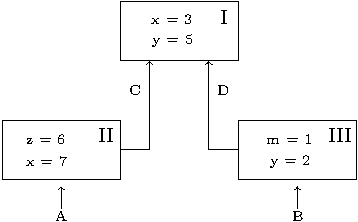
\includegraphics[width=250pt]{./images/frames.pdf}
\end{center}


An environment is made up of a linked chain of frames. Shown in
the figure are three frames, I, II, and III. Now, each of A, B, C,
and D are different environments, which view the frames in
different ways.

\begin{center}
\begin{tabular}{lrrll}
\toprule
Environment & x & y & z & m\\
\midrule
A & 7 & 5 & 6 & -\\
B & 3 & 2 & - & 1\\
C & 3 & 5 & - & -\\
D & 3 & 5 & - & -\\
\bottomrule
\end{tabular}
\end{center}

Environments can be considered as different ``vantage points'' of
the frame chain. From A, we see the values of the frame II and the
frames behind II, in this case I. Therefore, we get the values of
x, y, and z. However, there are two possible values of x. In this
case, we say that the value of x in frame II ``shadows'' the value
of x in all previous frames, and we consider that value to be the
correct one. Note that this is actually making the choice to use
the innermost scope's variables over ones in outer scopes. Other
environments are similarly analyzed. Note that C and D are the
same environment.

\subsection{Procedure Objects}
\label{sec:org6033d4c}

A procedure objects consists of:
\begin{enumerate}
\item A pointer to the procedure object.
\item A pointer to the environment the procedure will execute in.
\item The actual body (code) of the procedure.
\end{enumerate}

Diagrammatically:

\begin{center}
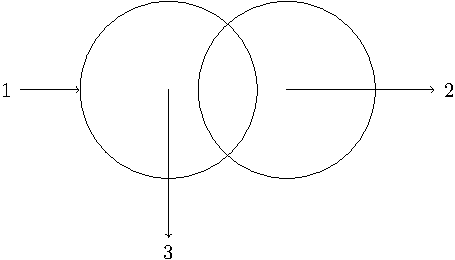
\includegraphics[width=200pt]{./images/frameobj.pdf}
\end{center}

\subsection{Rules for Environment Model}
\label{sec:org7589c2d}

\begin{enumerate}
\item A procedure object is applied to a set of arguments by
constructing a frame binding the formal parameters of the
procedure to the actual arguments of the call, then evaluating
the body of the procedure \emph{in the context} of the new
environment thus constructed. The new frame has as its
enclosing environment the environment part of the procedure
being applied.

For example, for a procedure \texttt{P}, evaluated at \texttt{(P 3 4)}, the
actual arguments to \texttt{P} are ``appended'' to the environment \texttt{P}
is called in. The procedure object itself has three pointers:

\begin{itemize}
\item The first is to the procedure itself, \texttt{P}.
\item The second points to the extended environment.
\item The third point points to the actual \(\lambda\).
\end{itemize}

Diagrammatically:

\begin{center}
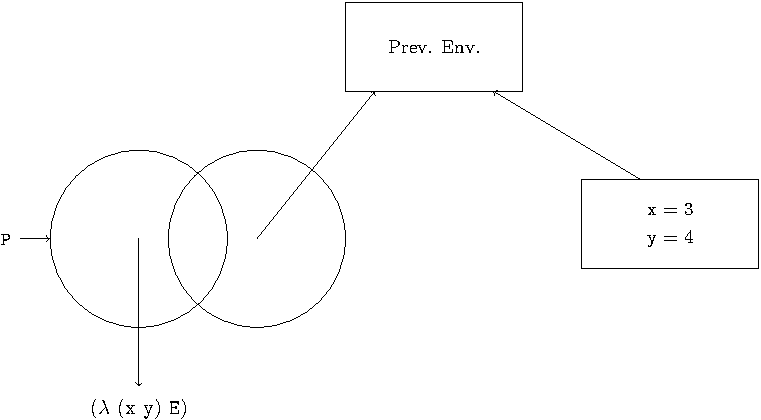
\includegraphics[width=300pt]{./images/rule1.pdf}
\end{center}

\item A \(\lambda\)-expression is evaluated relative to a given
environment as follows: a new procedure object is formed, the
combining the code of the \(\lambda\)-expression with a pointer to
the environment of evaluation.

This rule is self-explanatory.
\end{enumerate}

Our most important take-away is that an environment is a linked
chain of frames, going all the way back to the first (global)
frame. We now have a new working model, which works with
assignment, as we'll soon see.


\subsection{Assignment}
\label{sec:orgd30c397}

Let's play around with assignment in the environment model.
Consider the following procedure:

\begin{minted}[]{racket}
(define make-counter
  (lambda (n)
    (lambda ()
      (set! n (inc n))
      n)))
\end{minted}

What does the environment look like once we define \texttt{make-counter}?
Something like this:

\begin{center}
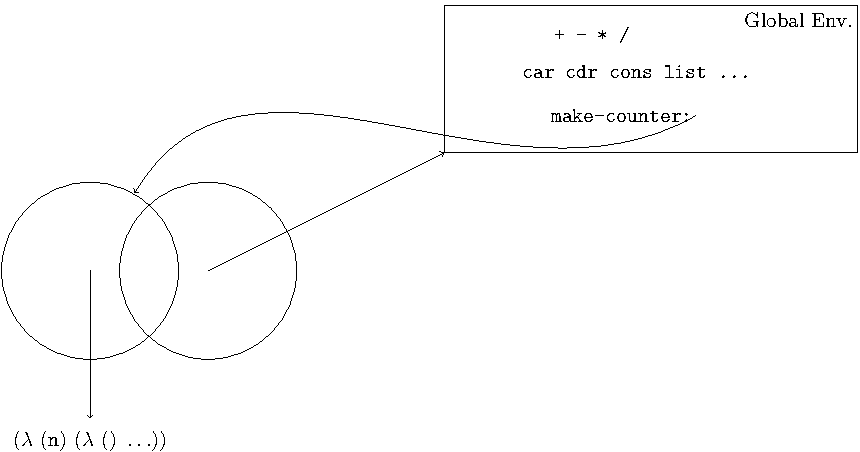
\includegraphics[width=0.8\textwidth]{./images/make-counter.pdf}
\end{center}

Let us now use \texttt{make-counter} to define two counters, each of
which start at different values of \texttt{n}:

\begin{minted}[]{racket}

(define C1 (make-counter 0))
(define C2 (make-counter 10))
\end{minted}

The environment now looks like:

\begin{center}
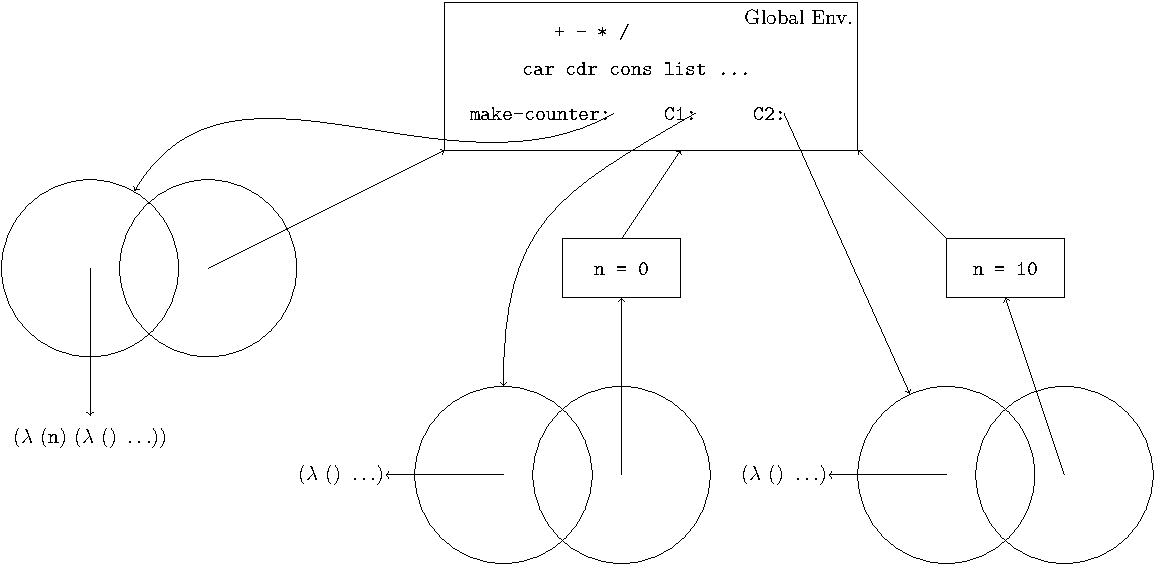
\includegraphics[width=0.95\textwidth]{./images/c1c2.pdf}
\end{center}

See that there is no \emph{possible} confusion between which \texttt{n} \texttt{C1}
uses and which \texttt{n} \texttt{C2} uses. Moreover, neither \texttt{C1} nor \texttt{C2}
would care about a globally defined \texttt{n}, or any \texttt{n} in a higher
level frame, since it'd get shadowed by their own \texttt{n}'s.

We can now see how the following would work:

\begin{minted}[]{racket}

(C1)
(C2)
(C1)
(C2)
\end{minted}

\begin{verbatim}
1
11
2
12
\end{verbatim}


The first call to \texttt{(C1)} sees that \texttt{n} is zero in its environment,
and sets \texttt{n} to \texttt{0+1=1}, and returns \texttt{1}. The first call to \texttt{(C2)}
sees that \emph{its} \texttt{n} is \texttt{10}, sets it to \texttt{11}, and returns \texttt{11}. The
second call to \texttt{(C1)} sees that its \texttt{n} is \texttt{1}, then sets and
returns \texttt{2}. The final call to \texttt{(C2)} sees that its \texttt{n} is \texttt{11},
which is then sets to \texttt{12} and returned.


\subsection{Some Philosophy}
\label{sec:org8b65425}

We have some questions to answer about sameness and change of
objects. Consider that in the previous example, \texttt{C1}'s \texttt{n} and
\texttt{C2}'s \texttt{n} are both called \texttt{n}, and yet refer to different
objects. However, \texttt{C1} refers to only one object, \texttt{C1}. How then,
can we tell if an identifier refers to an object? This issue is
almost philosophical: if the only way know of an object is its
identifier, what is an object anyway?

We avoid these issues in Lisp's environment model by defining
action, change, and identity as follows:

\begin{quote}
Action \(A\) has an effect on object \(X\) (\(A\) changes \(X\)) if
property \(P\) true of \(X\) before \(A\) is false of \(X\) after \(A\).
\end{quote}

and

\begin{quote}
\(X\) and \(Y\) are the same object if any action which changes \(X\)
changes \(Y\).
\end{quote}

The (Lisp) world is thus made up of many individual objects, all
with some local state.

\section{Advantages of Assignment}
\label{sec:orgcad46b5}

We've seen that introducing assignment makes our pure functional
programming somewhat ``murky''. One of the reasons to do this is that
assignment often greatly enhances modularity, as we will show in an
example. A word of caution, however: do not use assignment unless
it is necessary.

\subsection{Cesàro's Pi Finder}
\label{sec:org6eead8b}
Cesàro's theorem tells us that:

$$P(\mathrm{gcd}(a,b)=1) = \frac{6}{\pi^{2}}$$

Of course, we can estimate probabilities using the Monte Carlo
method (do lots of tests, and divide the number of successful tests
by the total number of tests conducted). Using assignment, the
program looks like:

\begin{minted}[]{racket}
(define (estimate-pi n)
  (sqrt (/ 6 (monte-carlo n cesaro))))

(define (cesaro)
  (= (gcd (random 4294967087) (random 4294967087)) 1))

(define (monte-carlo trials experiment)
  (define (iter remaining passed)
    (cond ((= remaining 0)
           (/ passed trials))
          ((experiment)
           (iter (dec remaining)
                 (inc passed)))
          (else
           (iter (dec remaining)
                 passed))))
  (iter trials 0))

(estimate-pi 10000000)
\end{minted}

\begin{verbatim}
3.141330429791511
\end{verbatim}


Note that we use Racket's built in \texttt{random} to generate a random
number. However, if we had to implement a PRNG on our own, it'd
look something like:

\begin{minted}[]{racket}
(define rand
  (let ((x random-init))
    (lambda ()
      (set! x (rand-update x))
      x)))
\end{minted}

Assignment is used most naturally here because we want to give \texttt{x}
the value of computing some function with input \texttt{x} to use the
next time \texttt{rand} is called. This function is evaluated within a
local scope where \texttt{x} at first has some constant seed value
\texttt{random-init}.


\subsection{Functional Cesàro's Pi Finder}
\label{sec:orgad7edda}

Since we can't use assignment to keep track of the ``state'' of the
PRNG, we must write our program like:

\begin{minted}[]{racket}
(define (estimate-pi n)
  (sqrt (/ 6 (random-gcd-test n))))

(define (random-gcd-test trials)
  (define (iter remaining passed x)
    (let ((x1 (rand-update x))
          (x2 (rand-update x1)))
      (cond ((= remaining 0)
             (/ passed trials))
            ((= (gcd x1 x2) 1)
             (iter (dec remaining)
                   (inc passed)
                   x))
            (else
             (iter (dec remaining)
                   passed
                   x2)))))
  (iter trials 0 random-seed))
\end{minted}

The state of the PRNG has ``leaked'' out into our program, that is,
\texttt{iter} has to keep track of successive values of the seed. Worse
still, this makes \texttt{monte-carlo} and \texttt{cesaro} non-general, reducing
modularity. It is applications like these where assignment is
incredibly useful, and helps keep our programs neat and modular.


























































































\chapter{Lecture 5B: Computational Objects}
\label{sec:org1bf0f62}

Now that we have local state, let's see what we can do with it. As
we saw earlier, real world objects also have local state. As such,
we can now make a model of the real world in our computer, taking
advantage of its inherent modularity to built a model with modular
objects.

We explore this possibility in this lecture by writing a simulator
for digital circuits in Lisp. Along the way, we'll have to implement
certain data structures which support local state.

\section{Digital Circuit Language}
\label{sec:org2f74cf8}

We build a language embedded in Lisp (in the same style as the
picture language) to simulate digital circuits. Here's the expected
usage:

\begin{minted}[]{racket}
(define a (make-wire))
(define b (make-wire))
(define c (make-wire))
(define d (make-wire))
(define e (make-wire))
(define s (make-wire))

(or-gate a b d)
(and-gate a b c)
(inverter c e)
(and-gate d e s)
\end{minted}

The \texttt{or-gate} takes two input wires \texttt{a} and \texttt{b}, and returns the
\texttt{OR} of the signals on wire \texttt{d}, very much like a real OR gate:

\begin{center}
\begin{circuitikz}
\draw (0,0) node[or port] (or) {}
(or.in 1) node[left=0.04cm](a) {A}
(or.in 2) node[left=0.04cm](b) {B}
(or.out) node[right=0.04cm](d) {D}
;
\end{circuitikz}
\end{center}

We could use these primitives to
write a half adder:

\begin{minted}[]{racket}
(define (half-adder a b s c)
  (let ((d (make-wire))
        (e (make-wire)))
    (or-gate a b d)
    (and-gate a b c)
    (inverter c e)
    (and-gate d e s)))
\end{minted}

\begin{center}
\begin{circuitikz}
\draw (0, 4)node[xor port] (xorone){}
(0, 2)node[and port] (and){}
(xorone.in 1) node[left=0.5cm](a) {A}
(xorone.in 2) node[left=0.5cm](b) {B}
(xorone.out) node[right=0.04cm](s) {S}
(and.out) node[right=0.04cm](c) {C}
(a.east) to[short,-*] (xorone.in 1) |- (and.in 1)
(b.east) to[short,-*] ($(b.east)!.5!(xorone.in 2)$) coordinate (branch)
-- (xorone.in 2)
(branch) |- (and.in 2);
\end{circuitikz}
\end{center}

Note carefully that the procedure \texttt{half-adder} doesn't actually
return anything: it merely makes calls to the gate procedures.
We'll see why later. Since the language is hierarchical, we could
now write a full adder:

\begin{minted}[]{racket}
(define (full-adder a b c-in sum c-out)
  (let ((s (make-wire))
        (c1 (make-wire))
        (c2 (make-wire)))
    (half-adder b c-in s c1)
    (half-adder a s sum c2)
    (or-gate c1 c2 c-out)))
\end{minted}

\subsection{Gates}
\label{sec:org58ab8e3}

Let us now implement the primitive gates of this language. Here's
an \texttt{inverter}:

\begin{minted}[]{racket}
(define (inverter in out)
  (define (invert-in)
    (let ((new
           (logical-not (get-signal in))))
      (after-delay inverter-delay
                   (lambda ()
                     (set-signal! out new)))))
  (add-action! in invert-in))
\end{minted}

\texttt{inverter} defines a procedure called \texttt{invert-in}, and adds that
action to the wire \texttt{in}. \texttt{invert-in} itself takes the logical not
of \texttt{in} and sets the signal on \texttt{out} to this value, after some
delay. See that this is precisely how a digital inverter in the
real world is expected to work: wires have certain signals
(\texttt{get-signal} and \texttt{set-signal}), these signals change according to
how the wires are routed \texttt{add-action!}, and there are certain
delays before the signal changes.

Of course, the primitive \texttt{logical-not} is easy to define:

\begin{minted}[]{racket}
(define (logical-not s)
  (cond ((= s 0) 1)
        ((= s 1) 0)
        (else
         (error "Invalid signal" s))))
\end{minted}

Similarly, \texttt{and-gate} can be defined as:

\begin{minted}[]{racket}
(define (and-gate a1 a2 out)
  (define (and-action-proc)
    (let ((new-value
           (logical-and (get-signal a1)
                        (get-signal a2))))
      (after-delay and-gate-delay
                   (lambda ()
                     (set-signal! out new-value)))))
  (add-action! a1 and-action-proc)
  (add-action! a2 and-action-proc))
\end{minted}

The only difference is in that we need to \texttt{get-signal} two signals
and \texttt{add-action!}'s to two signals. \texttt{logical-and} can be
implemented as:

\begin{minted}[]{racket}
(define (logical-and a b)
  (cond ((= a 0)
         (cond ((= b 0) 0)
               ((= b 1) 0)))
        ((= a 1)
         (cond ((= b 0) 0)
               ((= b 1) 1)))))
\end{minted}

Finally, an \texttt{or-gate} is implemented as:
\begin{minted}[]{racket}
(define (or-gate r1 r2 out)
  (define (or-action-proc)
    (let ((new-value
           (logical-or (get-signal r1)
                        (get-signal r2))))
      (after-delay or-gate-delay
                   (lambda ()
                     (set-signal! out new-value)))))
  (add-action! r1 or-action-proc)
  (add-action! r2 or-action-proc))
\end{minted}

\texttt{logical-or} is defined similar to \texttt{logical-and}:

\begin{minted}[]{racket}
(define (logical-or a b)
  (cond ((= a 0)
         (cond ((= b 0) 0)
               ((= b 1) 1)))
        ((= a 1)
         (cond ((= b 0) 1)
               ((= b 1) 1)))))
\end{minted}

\subsection{Wires}
\label{sec:org695c634}

We define wires as:

\begin{minted}[]{racket}
(define (make-wire)
  (let ((signal 0)
        (action-procs '()))
    (define (set-my-signal! new)
      (cond ((= signal new) 'done)
            (else
             (set! signal new)
             (call-each action-procs))))
    (define (accept-action-proc proc)
      (set! action-procs
            (cons proc action procs))
      (proc))
  (define (dispatch m)
    (cond ((eq? m 'get-signal) signal)
          ((eq? m 'set-signal!) set-my-signal!)
          ((eq? m 'add-action!) accept-action-proc)
          (else
           (error "Bad message" m))))
  dispatch))
\end{minted}

Clearly, a wire is defined by two local-scope variables, \texttt{signal}
and \texttt{action-procs}, which are initially set to \texttt{0} and \texttt{'()} (the
empty list, \texttt{nil}) respectively. Internally defined procedure
\texttt{set-my-signal!} does the obvious thing and sets the signal to the
new signal. It then calls all the action procedures of this wire.
\texttt{accept-action-proc} adds a new procedure to the front of the
existing action procedure list (\texttt{action-procs}) a new procedure.
It then calls this procedure for reasons we'll see later. Finally,
\texttt{dispatch} does the right thing according to its argument.

\texttt{call-each} is a simple \texttt{cdr} down a list and execution --- note the
extra parenthesis around \texttt{((car procs))}:

\begin{minted}[]{racket}
(define (call-each procs)
  (cond ((null? procs) 'done)
        (else
         ((car procs))
         (call-each (cdr procs)))))
\end{minted}

Naturally, we can now define \texttt{get-signal}, \texttt{set-signal}, and
\texttt{add-action} using the wire's \texttt{dispatch}:

\begin{minted}[]{racket}
(define (get-signal wire)
  (wire 'get-signal))

(define (set-signal! wire)
  (wire 'set-signal!))

(define (add-action! wire)
  (wire 'add-action!))
\end{minted}

\subsection{Delays}
\label{sec:orga2e2d8e}

We define the \texttt{after-delay} procedure as:

\begin{minted}[]{racket}
(define (after-delay delay action)
  (add-to-agenda!
   (+ delay (current-time the-agenda))
   action
   the-agenda))
\end{minted}

\texttt{after-delay} calls a function called \texttt{add-to-agenda!}.
\end{document}